\documentclass{article}

% if you need to pass options to natbib, use, e.g.:
%     \PassOptionsToPackage{numbers, compress}{natbib}
% before loading neurips_2021

% ready for submission
\usepackage[final]{neurips_2021}

%\usepackage[nonatbib]{neurips_2021}
%\usepackage[numbers]{natbib}

% to compile a preprint version, e.g., for submission to arXiv, add add the
% [preprint] option:
%     \usepackage[preprint]{neurips_2021}

% to compile a camera-ready version, add the [final] option, e.g.:
%     \usepackage[final]{neurips_2021}

% to avoid loading the natbib package, add option nonatbib:
%    \usepackage[nonatbib]{neurips_2021}

\usepackage[utf8]{inputenc} % allow utf-8 input
\usepackage[T1]{fontenc}    % use 8-bit T1 fonts
\usepackage{hyperref}       % hyperlinks
\usepackage{url}            % simple URL typesetting
\usepackage{booktabs}       % professional-quality tables
\usepackage{amsfonts}       % blackboard math symbols
\usepackage{nicefrac}       % compact symbols for 1/2, etc.
\usepackage{microtype}      % microtypography
\usepackage{xcolor}         % colors
\usepackage{wrapfig}

% custom imports
\usepackage{mystyle}
\usepackage{algorithm}
\usepackage[noend]{algorithmic}

\newcommand\todo[1]{\textcolor{red}{#1}}
\usepackage{subcaption}
\usepackage{multirow}


%\title{Embedded Structured Prediction}
%\title{Linearized Structured Models}
\title{Low-Rank Constraints for Fast Inference in Structured Models}

% The \author macro works with any number of authors. There are two commands
% used to separate the names and addresses of multiple authors: \And and \AND.
%
% Using \And between authors leaves it to LaTeX to determine where to break the
% lines. Using \AND forces a line break at that point. So, if LaTeX puts 3 of 4
% authors names on the first line, and the last on the second line, try using
% \AND instead of \And before the third author name.

\author{%
  Justin T. Chiu\thanks{Equal contribution}\\
  Cornell University \\
  \texttt{jtc257@cornell.edu} \\
  % examples of more authors
  \And
  Yuntian Deng\footnotemark[1] \\
  Harvard University \\
  \texttt{dengyuntian@seas.harvard.edu} \\
  \AND
  Alexander M. Rush \\
  Cornell University \\
  \texttt{arush@cornell.edu} \\
}

\begin{document}

\maketitle

\begin{abstract}
Structured distributions, i.e. distributions over combinatorial spaces, are commonly used to learn latent probabilistic representations from observed data. However, scaling these models is bottlenecked by the high computational and memory complexity with respect to the size of the latent representations. Common models such as Hidden Markov Models (HMMs) and Probabilistic Context-Free Grammars (PCFGs) require time and space quadratic and cubic in the number of hidden states respectively. This work demonstrates a  simple approach to reduce the computational and memory complexity of a large class of structured models. We show that by viewing the central inference step as a matrix-vector product and using a low-rank constraint, we can trade off model expressivity and speed via the rank.  Experiments with neural parameterized structured models for language modeling, polyphonic music modeling, unsupervised grammar induction, and video modeling show that our approach matches the accuracy of standard models at large state spaces while providing practical speedups.
\end{abstract}

\section{Introduction}

% structured prediction (lots of interesting tasks, general) and structured models (explicit dependencies across decisions)

When modeling complex sequential spaces, such as sentences, musical scores, or video frames,
a key choice is the internal structural representations of the model. A common choice in recent years is to use neural representations~\citep{nplm,mikolov-2011,gpt3,polyphonic,music-trans,video} to store a deterministic history. These models yield strong predictive accuracy but their deterministic, continuous forms provide little insight into the intermediate decisions of the model.

Latent structured models provide an alternative approach where complex modeling decisions are broken down into a series of probabilistic steps. Structured models provide a principled framework for reasoning about the probabilistic dependencies between decisions and for computing posterior probabilities. 
%The structure of the decision processes also affords opportunities for interpretability and controllability through probabilistic inference \citep{pgm,levine2018reinforcement}.
% ^ posterior inference allows for interp+control, the "also" makes it sound like it is orthogonal
The structure of the decision processes and the ability to answer queries through probabilistic inference afford interpretability and controllability that are lacking in neural models~\citep{pgm,levine2018reinforcement}.
 
%modeling rich and interdependent output variables.
%such as those that are found in language modeling \citep{nplm,mikolov-2011,gpt3}, polyphonic music generation \citep{polyphonic}, and video modeling \citep{video,fried2020learning}.
%Structured models, which explicitly reason about the dependencies between variables, have long been the backbone of structured prediction methods.

% inference expensive
Despite the benefits of structured models, the computational complexity of training scales asymptotically much worse than for neural models, as inference, and therefore training, requires marginalizing over all possible latent structures.
For standard general-purpose models like Hidden Markov Models (HMM) and Probabilistic Context-Free Grammars (PCFG), the runtime of inference scales quadratically and cubically in the number of states respectively, which limits the ability to reach a massive scale.
Promisingly, recent work has shown that in specific situations these models can be scaled, and that the increased scale results in commensurate improvements in accuracy -- without sacrificing the ability to perform exact inference~\citep{dedieu2019learning,chiu2020scaling,yang2021pcfgs}.

In this work, we propose an approach for improving the runtime of a large class of structured latent models by introducing a low-rank constraint. 
We target the family of models where inference can be formulated through a
labeled directed hypergraph, which describes a broad class
of dynamic-programming based inference~\citep{klein2004parsing,huang2005better,zhou2006learning,javidian2020hypergraph,chiang2020factor}. We show how under low-rank constraints these models allow for more efficient inference. 
Imposing a low-rank constraint allows for a key step of inference to be rewritten as a fast matrix-vector product.
This approach is also inspired by recent advances in computationally efficient neural attention  attention~\citep{katharopoulos2020lineartransformer,peng2021rfa,choromanski2020performer},
a significantly different task and formulation, that also uses  rewrites matrix-vector products as fast low-rank products using a approximate kernel techniques.

We evaluate this approach by learning low-rank structured models for the tasks of language modeling, polyphonic music modeling, unsupervised grammar induction, and video modeling. For these tasks we use a variety of models including HMMs, PCFGs, and Hidden Semi-Markov Models (HSMMs).
As the application of low-rank constraints is nontrivial in high-dimensional structured models due to reduced expressivity, we demonstrate effective techniques for overcoming several practical challenges of low-rank parameterizations.
We find that our approach achieves very similar results to unconstrained models at large state sizes, while the decomposition allows us to greatly increase the speed of inference.
Results on HMMs show that we can scale to more than 16,000 states; results on PCFGs achieve a significant perplexity reduction from much larger state spaces compared to past work \citep{kim2019cpcfg}; and results on HSMMs show that our formulation enables scaling to much larger state spaces for continuous emissions~\citep{fried2020learning}.

\section{Latent Structure and Hypergraphs}

We consider the problem of modeling a sequence of observations $p(x)= p(x_1, \dots, x_T)$.
These observations can range in complexity from the words in a sentence to a series of co-occurring musical notes,
or to features of video frames, and 
may be discrete or continuous.
We assume these observations are generated by an unobserved (latent) structured representation $z$, and therefore model the joint
$p(x, z)$.
The structure may be sequential or hierarchical, such as latent trees,
and the set of structures $\mcZ$ is combinatorial, i.e. exponential in size with respect to the input sentence. 
In order to train these models on observations, we must optimize the evidence
$p(x) = \sum_z p(x,z)$ by marginalizing over $z$. Scaling this marginalization is the focus of this work. 

% Models of interest
Hypergraphs are a graphical model formalism  for structured distributions that admit tractable
inference through dynamic programming~ \citep{klein2004parsing,huang2005better,zhou2006learning,javidian2020hypergraph,chiang2020factor}.\footnote{While the formalism is similar to undirected factor graphs,
it allows us to represent more complex distributions: notably
dependency structures with unknown topologies, such as latent trees.}
Define a labeled, directed, acyclic hypergraph as a set of nodes
$\cal V$, a set of hyperedges $\cal E$, and a designated root node $S \in {\cal V}$. 
Each node $v \in \mcV$ has a collection of labels ${\cal L}_v$.
Each hyperedge $e\in\mcE$ consists of a head node $u$ and tuple of tail nodes, $v = (v_1, \ldots, v_{|e|})$, where $|e|$ is the number of tail nodes.
For simplicity, we will assume \textit{at most} 2 tail nodes $v_1, v_2$, and unless noted, a fixed label set $\mcL$ throughout.
Each hyperedge $e$ is associated with a score matrix $\Psi_e\in\R^{\mcL\times \mcL^{|e|}}$ 
with a score for all head and tail labels.\footnote{This formalism can represent inference in both locally and globally normalized models, although we focus on local normalization in this work.}
We use the notation $[\Psi_e]_{z_u,(z_1, z_2)}$ to indicate the score for head label $z_u$ and tail labels $z_1$ and $z_2$.
Finally, we assume we have a topological ordering over the edges.

A hypergraph is used to aggregate marginals bottom-up, which is done through a dynamic programming (belief propagation) algorithm. 
Algorithm~\ref{lab:hyp-matrix}~(left) shows the algorithm. It works by filling in a table vector 
$\alpha_v \in \R^{\mcL}$ for each node $v$ in order, and is initialized to 1 at the leaf nodes.\footnote{
The accumulation of scores is denoted by $\stackrel{+}{\gets}$.
Multiple hyperedges can have the same head node, whose scores must be added together.}
It returns the sum over latent structures, $p(x)$. Counting
loops, the worst-case runtime complexity is
$O(|{\cal E}|\times L^{|e^*|+1})$ where $L = |{\cal L}|$ is the size of the
label set and $|e^*|$ the max hyperedge tail size. Algorithm~\ref{lab:hyp-matrix}~(right) shows the 
same algorithm in matrix form by introducing joined tail vectors $\beta_v\in\R^{\mcL^{|e|}}$ for each group of nodes $v$.  Letting $z_v = (z_1,z_2)$, the joined tail vector contains entries $[\beta]_{z_v} = [\alpha_{v_1}]_{z_1}[\alpha_{v_2}]_{z_2}$.

\begin{algorithm}[t]
\begin{minipage}[t]{0.50\textwidth}
\begin{algorithmic} 
\STATE{[\textit{Scalar Form}]}
\FOR {$u \leftarrow v_1, v_2$ hyperedge $e$ topologically}
\FOR {$z_u \in {\cal L}_u$ }
%\STATE $[\alpha_u]_{z_u} \stackrel{+}{\gets}  \displaystyle \sum_{z_1, z_2}  [\Psi_e]_{z_u,(z_1, z_2)}$
\STATE $[\alpha_u]_{z_u} \stackrel{+}{\gets}  \sum_{z_1, z_2}  [\Psi_e]_{z_u,(z_1, z_2)}$
\STATE \hspace{7em} $\bm\cdot \ [\alpha_{v_1}]_{z_1} \  [\alpha_{v_2}]_{z_2}$
\ENDFOR
\ENDFOR
\STATE \textbf{return} $\sum_z [\alpha_S]_z$
\end{algorithmic}
%\end{algorithm}
\end{minipage}
%\hspace{.5em}
\begin{minipage}[t]{0.45\textwidth}
%\begin{algorithm}[H]
\begin{algorithmic} 
\STATE{[\textit{Matrix Form}]}
\FOR {$u \leftarrow v$ hyperedge $e$ topologically}
\STATE $\alpha_u \stackrel{+}{\gets} \Psi_e\beta_v$
\ENDFOR
\STATE \textbf{return} $\alpha_S^\top \mathbf{1}$

\vspace{1.5em}
\end{algorithmic}
\end{minipage}
\caption{\label{lab:hyp-matrix} Hypergraph marginalization }
\end{algorithm}

To make this formalism more concrete, we show how hypergraphs can be used for inference in several structured generative models: hidden Markov models,  probabilistic context-free grammars, and hidden semi-Markov models.
Inference in these examples are instances of the hypergraph algorithm.

\textbf{Example: Hidden Markov Models (HMM)}
HMMs are discrete latent sequence models defined by the following generative process: first, a sequence of discrete latent states $z = (z_1, \ldots,z_T)$ with state size $L$ are sampled as a Markov chain. Then each state $z_t$ independently emits an observation $x_t$, i.e. 
\begin{equation}
\label{eqn:hmm}
    p(x,z) = \prod_{t=1}^T p(z_t \mid z_{t-1})\ p(x_t\mid z_t),
\end{equation}
where $p(z_t \mid z_{t-1})$ is the transition distribution,
 $p(x_t \mid z_t)$ the emission distribution, and $p(z_1 \mid z_0)$ is the initial distribution with distinguished start symbol $z_0$.

Given a sequence of observations $x=(x_1, \ldots, x_n)$ we can compute
$p(x) = \sum_zp(x,z)$ using a labeled directed hypergraph, with single-tailed edges, nodes corresponding to state positions, labels corresponding to states, and emissions probabilities incorporated into the scoring matrices $\Psi$.
There are $T$ scoring matrices, $\Psi_t\in\R^{\mcL\times\mcL}$, with entries $[\Psi_t]_{z_t,z_{t+1}} = p(z_{t+1},x_t \mid z_t)$ corresponding to transitions.\footnote{
The left-most scoring matrix for the HMM has entries $[\Psi_1]_{z_1,z_{2}} = p(z_{2},x_1 \mid z_1)p(z_1\mid z_0)$.
}
Algorithm~\ref{fig:marg-hmm-pcfg}~(left) shows the approach. This requires time $O(TL^2)$ and is identical to the backward algorithm for HMMs.\footnote{
In the case of HMMs, the table vectors $\alpha_t$ correspond to the backward algorithm's $\beta$ values.}

\begin{algorithm}[t]
\caption{Hypergraph marginalization for HMMs and PCFGs}
\label{fig:marg-hmm-pcfg}
\begin{minipage}[t]{0.45\textwidth}
%\small
\begin{algorithmic}
\STATE {[\textit{HMM - Backward}]}
\FOR {$t \leftarrow (t+1)$ in right-to-left order}
\FOR {$z_{t+1} \in \mcL$}
\STATE $[\beta_{t+1}]_{z_{t+1}} = [\alpha_{t+1}]_{z_{t+1}}$
\ENDFOR
\STATE $\alpha_t \stackrel{+}{\gets} \Psi_t \beta_{t+1}$
\ENDFOR
\STATE \textbf{return} $\alpha_0^\top \mathbf{1}$
\end{algorithmic}
\end{minipage}
\vspace{0pt}
\begin{minipage}[t]{0.50\textwidth}
%\small
\begin{algorithmic} 
\STATE {[\textit{PCFG - CKY}]}
\FOR {$(i,k) \leftarrow (i,j), (j,k)$ in span-size order}
\FOR {$z_1,z_2 \in \mcL_{i,j}\times\mcL_{j,k}$}
\STATE $[\beta_{i,j,k}]_{(z_1,z_2)} = [\alpha_{i,j}]_{z_1}[\alpha_{j,k}]_{z_2}$
\ENDFOR
\STATE $\alpha_{i,k} \stackrel{+}{\gets} \Psi\beta_{i,j,k}$
\ENDFOR
\STATE \textbf{return} $\alpha_{1,T}^\top \mathbf{1}$
\end{algorithmic}
\end{minipage}
\end{algorithm}

%\end{comment}


\textbf{Example: Context-Free Grammars (CFG)}
CFGs are a structured model defined by the 5-tuple 
$\mcG = (S,\mcN,\mcP,\mcX,\mcR)$, where $S$ is the distinguished start symbol, $\mcN$ is a set of nonterminals, $\mcP$ is a set of preterminals, $\mcX$ is the token types in the vocabulary, and $\mcR$ is a set of grammar rules.
Production rules for start, nonterminals, and preterminals take the following forms:\footnote{
We restrict our attention to grammars in Chomsky normal form.}
\begin{equation}
\label{eqn:pcfg-rules}
\begin{aligned}
S&\to A, & A\in\mcN; &&
A&\to B\ C, & B,C\in\mcN\cup\mcP; &&
D&\to x, & D \in\mcP,x\in\mcX.
\end{aligned}
\end{equation}
A probabilistic context-free grammar (PCFG) additionally has a probability measure on the set of rules.
To compute $p(x_1, \ldots, x_T)$ with a hypergraph, we create one node for each contiguous
 subspan $[i, k)$ in the sentence. Nodes with $i + 1 < k$ have a
nonterminal label set ${\cal L} = \mcN$. Nodes with $i + 1=k$ have a 
preterminal label set ${\cal L}_{i,i+1} = \mcP$.
%We first initialize the scores of preterminals for spans of size 1, $\alpha_{i,i+1}$, with entries $[\alpha_{i,i+1}]_{z} = p(x_i\mid z)$ for each $i \in 1,\ldots,T$ and $z \in \mcP$.
%For the rest of the algorithm, we focus on the hyperedges for nonterminal productions, as those dominate the runtime.
The main scoring matrix is $\Psi\in\R^{\mcL\times \mcL^2}$, with entries $[\Psi]_{z_u,(z_1,z_2)} = p(z_1,z_2\mid z_u)$.\footnote{We have a separate matrix for terminal production on $x$ which we elide for 
simplicity.}
Algorithm~\ref{fig:marg-hmm-pcfg} (right) shows how for every hyperedge we join the scores from the two tail nodes in $\alpha_{i,j}$ and $\alpha_{j,k}$ into joined tail vector $\beta_{i,j,k}\in\R^{\mcL^2}$. %This contrasts with HMMs, which only have a single tail node per hyperedge and therefore do not require joining.
As there are $O(T^3)$ hyperedges and the largest ${\cal L}$ is of size
$|\mcN|$, the runtime of the algorithm is $O(T^3 {|\mcN|}^3)$. This approach is identical to the CKY algorithm.

% do we need this?
\textbf{Example: Hidden Semi-Markov Models (HSMM)}
HSMMs are extensions of HMMs that allow for generating a variable-length sequence of observations per state. 
It defines the following generate process: first, we sample a sequence of discrete latent states $z=(z_1, \cdots, z_K)$ with a first-order Markov model. We then use them to generate the length of observations per state. For our experiments we generate independent continuous emissions $x_t$ with a Gaussian distribution for $p(x_i\mid z_k)$. Full details of the inference procedure are given in Appendix~\ref{sec:hsmm}.

% It defines the following generate process: first, we sample a sequence of discrete latent states $z=(z_1, \cdots, z_K)$ with a first-order Markov model. A notable difference from HMMs is that we sample variable-length sequences as opposed to a fixed length sequence, by introducing a special end-of-sequence state. Next, we sample the length of observations under each state from a Poisson distribution $l_k\sim \text{Poisson}(\lambda_{z_k})$ truncated at max length $M$. The joint distribution is defined as
% \begin{equation}
% \label{eqn:hsmm}
%     p(x, z, l) = \prod_{k=1}^K p(z_k \mid z_{k-1}) \ p(l_k \mid z_k)\prod_{i=l_1+\cdots+l_{k-1}}^{l_1+\cdots+l_k} p(x_i\mid z_k),
% \end{equation}
% where the sequence length $T$ can be computed as $T=\sum_{k=1}^K l_k$. In this work, we only consider modeling continuous $x_t$, so we use a Gaussian distribution for $p(x_i\mid z_k)$.

% To compute $p(x)$, we can marginalize $l, z$ using dynamic programming similar to HMMs, except that we have an additional factor of $M$: the overall complexity is $O(T\times M \times L^2)$ (ignoring the emission part since they are usually not the bottleneck). We refer to \citet{yu2010hidden} for more details.

\section{Rank-Constrained Structured Models}
\label{sec:linearizing}

For these structured distributions, hypergraphs provide a general method for inference (and therefore training parameterized versions). However, the underlying algorithms scale poorly with the size of the label sets (quadratic for HMM and HSMM, cubic for CFG). This complexity makes it challenging to scale these models and train versions with very large numbers of states.

In this section, we consider an approach for improving the scalability
of these models by reducing the dependence of the computational complexity of inference on the label set size.
The main idea is to speed up the matrix-vector product step in inference by using a low-rank decomposition of 
a scoring matrix $\Psi$.
%This is accomplished by imposing a constraint on the scoring functions which determine the entries of $\Psi$.
In the next section we show that this constraint can easily be incorporated into parameterized versions of these models.

%\subsection{Kernelizing Hyperedges}
\subsection{Fast Matrix-Vector Products}
The main bottleneck for inference speed is the matrix-vector product $\alpha_u = \Psi_e\beta_v$ that must be computed for every edge in the hypergraph.
As we saw in Algorithm~\ref{lab:hyp-matrix} (left), this step takes time $L^{|e|+1}$ to compute,
which can immediately be sped up by making structural assumptions
on $\Psi_e$.
%However, the matrix form Algorithm~\ref{lab:hyp-matrix} (right) hints that there is an alternative way to view this computation as a kernel.

We note the following elementary property of matrix-vector products.
If the scoring matrix can be decomposed as the product
of two rank-$N$ matrices $\Psi_e = U_e V_e^\top$,
i.e. a low-rank decomposition,
then the matrix-vector products can be computed in time
$O(|{\cal E}|\times L^{|e|}\times N)$,
exchanging a factor of $L$ for a factor of $N$.
This leads to the following matrix-vector product expression for each hyperedge $e$ with $u\leftarrow v$:
\begin{equation}
    \label{eqn:hypergraph-update-kernel-matrix}
    \Psi_e\beta_v =  \left(U_e V_e^\top\right) \beta_v =  U_e\left(V_e^\top\beta_v\right).
\end{equation}

Unfortunately, not every parameterization of scoring matrices $\Psi_e$
admits an exact low-rank decomposition.
The most common parameterization, softmax, uses
exponential kernels~\citep{tsai2019kernelattn}, $$[\Psi_e]_{z_u,(z_1,z_2)} \propto 
    \exp(f(z_u), g(z_1,z_2)) = K_\SM(f(z_u), g(z_1, z_2)),$$ 
which does not admit an exact low-rank decomposition or linearization~\citep{steinwart2006explicit}.\footnote{
While the exponential kernel does not afford an exact linearization, the kernel can be approximated deterministically \citep{cotter2011approx} or stochastically \citep{rahimi2007rff}.
The stochastic approximation is a key component of recent work on efficient attention \citep{choromanski2020performer,peng2021rfa}.}.
We instead restrict out attention to nonnegative feature mappings\footnote{The nonnegative feature mapping ensures that the resulting scoring matrix $\Psi$ is a valid probability distribution.} $\phi:\R^D\to\R^N_+$ \citep{choromanski2020performer}, such that
\[[\Psi]_{z_u, (z_1, z_2)} = c_{z_u} c_{z_1,z_2} \phi(f(z_u))^\top\phi(g(z_{1}, z_{2})) = K(f(z_u), g(z_1, z_2)),  \]
where $c_{z_u},c_{z_1,z_2}$ contain normalizing constants and clamped potentials (e.g. conditional probabilities), and we use $v = (z_1,z_2)$ for brevity.
We refer to $K$ with a low-dimensional nonnegative feature mapping
as an efficiently linearizable kernel.
We then have
\begin{equation}
    [U_e]_{z_u,n} = c_{z_u}[\phi(f(x_u))]_n 
    \qquad
    [V_e]_{(z_1,z_2),n} = c_{z_1,z_2} [\phi(g(z_1,z_2))]_n.
\end{equation}
Algorithm~\ref{alg:low-rank-update} shows the role of the low-rank
matrix-vector product in marginalization.\footnote{
If the normalizing constants are given by $c_{z_u}$,
they can be computed from unnormalized $\tilde{U}_e,\tilde{V}_e$ as follows: $c_{z_u} = [\tilde{U}_e\tilde{V}_e^\top\mathbf{1}]_{z_u}$ in time $O(L^{|e|}N + LN)$, and similarly for $c_{z_1,z_2}$.
}
In practice, low-rank constraints can result in significant speedups. For instance, HMMs and HSMMs go from scaling quadratically
in the number of hidden states to linearly (with a new factor of the
feature dimension).

\begin{wrapfigure}{r}{0.55\textwidth}
\begin{minipage}{0.55\textwidth}
\begin{algorithm}[H]
%\begin{comment}
\caption{\label{alg:low-rank-update} Low-rank marginalization}
\begin{algorithmic} 
\FOR {$u \leftarrow v_1, v_2$ hyperedge $e$ topologically}
\FOR {$n \in 1,\ldots,N$}
%\STATE $[\beta]_n \gets \sum_{z_1, z_2} c_{z_1, z_2}\  [\phi(g(z_{1}, z_{2}))]_n \  \alpha_{v_1}(z_1) \  \alpha_{v_1}(z_2)$
    %\hfill $\vartriangleright$ $O(\mcL^{|e|} N)$
\STATE \hspace*{-0.2cm}$[\gamma]_n = \displaystyle \sum_{z_v} c_v\  [\phi(g(z_{1}, z_{2}))]_n \  [\beta_{v}]_{z_v}$
\hfill $\vartriangleright$ $O(L^{|e|})$
\ENDFOR
\STATE $\alpha_u \stackrel{+}{\gets} U_e\gamma $
    \hfill $\vartriangleright$ $O(LN)$
\ENDFOR
\STATE \textbf{return} $\alpha_S^\top\mathbf{1}$
\end{algorithmic} 
\end{algorithm}
\end{minipage}
\end{wrapfigure}

\subsection{Application to Structured Models}
As enforcing a low-rank factorization in every conditional distribution limits the expressivity of a model,
we explicitly target distributions that are involved in computational bottlenecks.\footnote{For a discussion of the expressivity of low-rank models compared to models with fewer labels, see Appendix~\ref{sec:expressivity}.}
For these key distributions, we use an efficiently linearizable kernel $K$, allowing factorization of the scoring matrix.
For other computations, we utilize a standard softmax kernel $K_\SM$ and do not factorize the resulting scoring matrix.
We refer to this as a mixed parameterization.

\textbf{Hidden Markov Models}
Low-rank HMMs (LHMMs) use the following mixed kernel parameterization, which specifically targets the state-state transition bottleneck:
\begin{equation}
\begin{aligned}
p(z_1 \mid z_0) &\propto K(\bu_{z_0}, \bv_{z_1}),&
p(z_t \mid z_{t-1}) &\propto K(\bu_{z_{t-1}}, \bv_{z_t}),&
p(x_t \mid z_t) &\propto K_\SM(\bu_{z_t}, \bv_{x_t}),
\end{aligned}
\end{equation}
where $\bu_{z}$ is the embedding of the head label and $\bv_{z}$
the embedding of the tail label. 
This allows $\Psi$ to be decomposed as the $p(x_t\mid z_t)$ terms become constants.
The embeddings come from neural network parameterizations detailed in Appendix~\ref{sec:mlp-param}.

This allows inference to be run in time $O(TLN)$, where $T$ is the length of a sequence, $L$ the size of the label space, and $N$ the feature dimension.

\textbf{Hidden Semi-Markov Models}
The low-rank HSMM (LHSMM) uses a similar kernel parameterization:
\begin{equation}
\label{eqn:hsmm}
\begin{aligned}
p(z_1 \mid z_0) &\propto K(\bu_{z_0}, \bv_{z_1}),&
p(z_k \mid z_{k-1}) &\propto K(\bu_{z_{k-1}}, \bv_{z_k}),&
p(x_t \mid z_k) &\propto K_{\text{Gauss}}(\bu_{z_k}, \mathbf{x}_t),
\end{aligned}
\end{equation}
where $K_{\text{Gauss}}(\cdot, \cdot)$ is the Gaussian kernel used to model continuous $\mathbf{x}_t$. The total inference complexity is $O(TLMN )$, where $M$ is the maximum length of the observation sequence under any state.

\textbf{Context-Free Grammars}
The PCFG uses a similar mixed parameterization to the HMM.
These probabilities correspond to start ($S\to A$), preterminal ($D\to x$),
and standard productions ($A\to B\ C$) respectively.
\begin{equation}
\label{eqn:pcfg}
\begin{aligned}
p(z_{1,N} \mid S ) &\propto K_\SM(\bu_{S}, \bu_{z_{1,N}}),&
p( z_{i,j}, z_{j,k} \mid z_{i,k}) &\propto \begin{cases}
  K_\SM(\bu_{z_{i,k}}, \bv_{z_{i,j}\ z_{j,k}}) & \substack{i+1 = j \lor \\j+1=k} \\ 
 K(\bu_{z_{i,k}}', \bv_{z_{i,j}\ z_{j,k}}) &\text{o.w.} \\
\end{cases}\\
 p(x_i \mid z_i) &\propto K_\SM(\bu_{z_i}, \bv_{x_i}),\\
\end{aligned}
\end{equation}
where $\bu_{z}$/$\bu_z'$ is the embedding of $z$ when $z$ is used as head,$\bv_{x}$/$\bv_{z_1, z_2}$ is the embedding of $x$/$(z_1, z_2)$ when they are used as tail. See Appendix~\ref{sec:mlp-param} for the full
parameterization, drawn from \citet{kim2019cpcfg}. Note that we limit
the application of low-rank constraints to nonterminal to nonterminal
productions. These productions dominate the runtime as they
are applied at $O(T^3)$ hyperedges.

This allows inference to be run in time $O(T^3L^2N)$, where $T$ is the length of a sequence, $L$ the size of the label space, and $N$ the feature dimension.


\section{Experimental Setup}
\label{sec:experiments}
We evaluate the application of low-rank constraints with four experiments: sequential language modeling with HMMs, polyphonic music modeling with a large observation space, hierarchical language modelings with PCFGs, and video modeling with HSMMs.

\textbf{Data}
Our first set of experiments evaluate sequential models on \textsc{Penn Treebank} dataset (\textsc{Ptb}) \citep{ptb} for the task of word-level language modeling.
%For our experiments with HMMs for language modeling,
We use the preprocessing from \citet{mikolov-2011}. The second set of experiments is on polyphonic music modeling \citep{polyphonic}.
We evaluate on four music datasets: Nottingham (Nott), Piano, MuseData (Muse), and JSB chorales (JSB).
Each timestep consists of an 88-dimensional binary vector indicating whether a particular note is played. Since multiple notes may be played at the same time, the effective vocabulary size is extremely large. The third set of experiments use PCFGs for language modeling, we also use \textsc{Ptb}, but with the splits and preprocessing used in unsupervised constituency parsing \citep{shen2018prpn,shen2018ordered,kim2019cpcfg}. The last set of experiments use HSMMs for video modeling, where we use \textsc{CrossTask} \citep{zhukov2019cross} with 10\% of the training data for validation. We follow the preprocessing steps in \citet{fried2020learning} and apply PCA to project features to vectors of size 200. For the full data details, please see Appendix~\ref{sec:data}.

\textbf{Models and Hyperparameters}
%\begin{comment}
%The categorical experiments use vectors of dimension 128 for both the model and the true distribution.
%For the model, we use the $\phi_{\textrm{pos}}$ feature map.
%We initialize the model parameters in the categorical experiments with $\bu_q,\bv_k\sim\Unif(-\gamma,\gamma)$ where $\gamma=0.001$, and then normalize them to have $l_2$ norm 1.
%and train via gradient descent with a learning rate of 1 for 30k updates.
%\end{comment}
For language modeling with HMMs, we experiment with a range of state sizes, $|\mcL| = L \in \set{2^{10}, 2^{11}, 2^{12}, 2^{13}, 2^{14}}$,
and rank $N \in \set{L/2, L/4, L/8}$.
For polyphonic music modeling with HMMs, we experiment with states sizes $L \in \set{2^7, 2^8, 2^9, 2^{10}, 2^{11}}$.
For language modeling with PCFGs, we use a set of nonterminals of size $|\mcN| \in \set{30, 60, 100}$ and preterminals of twice the number of nonterminals $|\mcP|=2|\mcN|$. Our smallest setting ($|\mcN|=30$, $|\mcP|=60$) is the one used in \citet{kim2019cpcfg}. For video modeling with HSMMs, we use the same model setting as \citet{fried2020learning}, but we don't constrain states to the predefined states per task, and we experiment with state sizes $L \in \set{2^6, 2^7, 2^8, 2^9, 2^{10}}$ and rank $N \in \set{2^4, 2^5, 2^6, 2^7}$.

We utilize the feature map $\phi(x) = \exp(Wx)$ for the LHMM and LHSMM, and $\phi(x) = \exp(Wx - \|x\|_2^2/2)$ for the LPCFG. We initialize the parameters of feature maps using orthogonal feature projections \citep{choromanski2020performer}, and update it alongside the model parameters.
For the full hyperparameter and optimization details, see Appendix~\ref{sec:opt}.

\textbf{Baselines and Evaluation}
The language modeling experiments are evaluated using perplexity. Baselines are neurally parameterized HMM
with a standard softmax transition.  We also compare to VL-HMM, which makes a strong structural sparsity assumption on the emission distribution~\citep{chiu2020scaling}. We include for reference a state-of-the-art language model, the AWD-LSTM~\citep{merity2017awdlstm}. For polyphonic music modeling, we compare our LHMM against RNN-NADE~\citep{polyphonic} which models the full joint distribution of notes as well as temporal dependencies; as well as autoregressive neural models such as the R-Transformer~\citep{rtransformer} (as reported by \citet{betalstm}) and an LSTM ~(as reported by \citet{flow}); models with latent continuous dynamics such as the LV-RNN \citep{nasmc} and SRNN \citep{srnn}; and finally comparable models with latent discrete dynamics, the TSBN \citep{tsbn} and the baseline HMM.
%As the preprocessing of \textsc{Ptb} for the PCFG language modeling differs from that of \citet{mikolov-2011}, perplexities reported on the two datasets are incomparable. 
We evaluate perplexities of our low-rank PCFG (LPCFG) against a softmax PCFG (PCFG) \citep{kim2019cpcfg}. For video modeling, we evaluate the negative log likelihoods on the test set and compare low-rank HSMMs to softmax HSMMs.

\begin{comment}
\begin{figure*}
 \begin{subfigure}[t]{0.47\textwidth}
  \centering
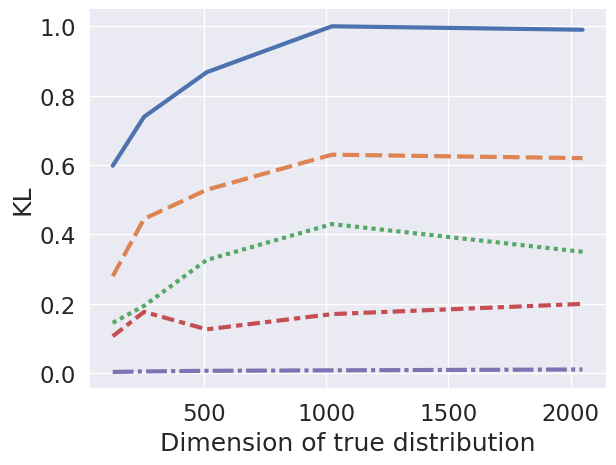
\includegraphics[height=4.5cm]{imgs/hmm/cat-kl.png}
\caption{}
\end{subfigure}
\begin{subfigure}[t]{0.43\textwidth}
\centering
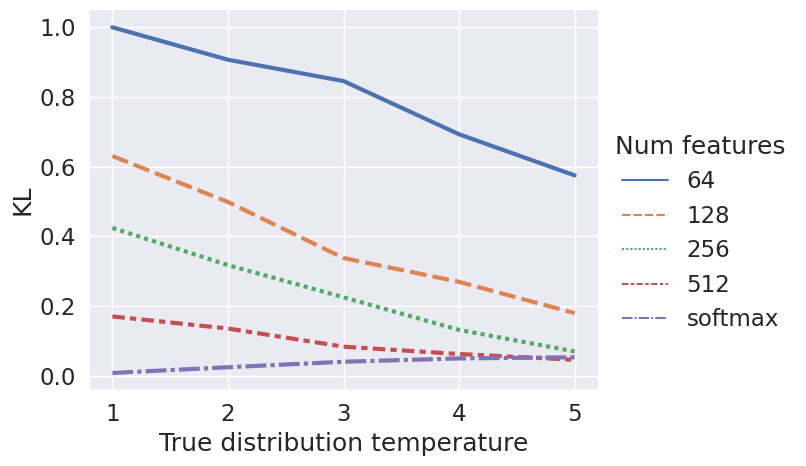
\includegraphics[height=4.5cm]{imgs/hmm/cat-temp-kl.png}
\caption{}
\end{subfigure}
\caption{\label{fig:cat-kl}The KL between the true synthetic categorical distribution and learned low-rank model, measuring the effect of: (a) The dimension of the true distribution $|\mcL|$. The number of queries is held constant at 128 and temperature at $\tau=1$, while the dimension of the true distribution 
and the number of features in the low-rank model is varied. (b) The temperature of the true distribution $\tau$. The number of queries is held constant at 128 and keys at 1024, while the temperature of the true distribution 
and the number of features is varied.}
\end{figure*}
\end{comment}

\section{Results}\label{sec:results}

\textbf{Hidden Markov Models for Language Modeling}
\begin{figure}[t]
\begin{subfigure}[t]{0.40\textwidth}
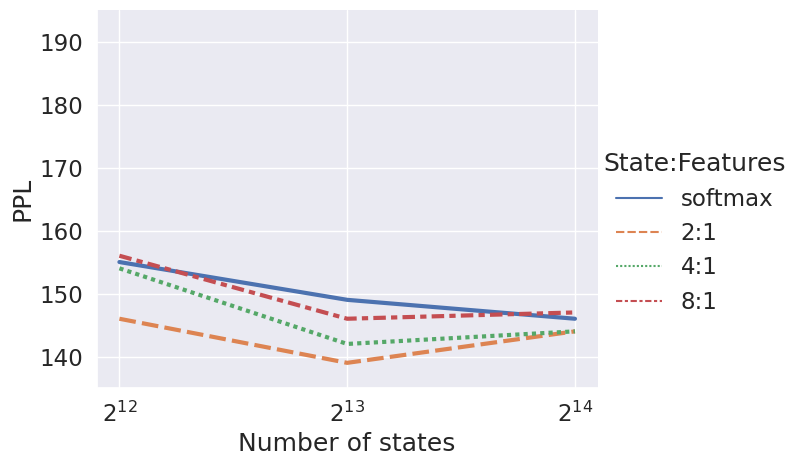
\includegraphics[height=4.5cm,trim={0 0 5cm 0}, clip]{imgs/hmm/lhmm-states-features-dropout.png}
\end{subfigure}
\hspace{1.5em}
\begin{subfigure}[t]{0.50\textwidth}
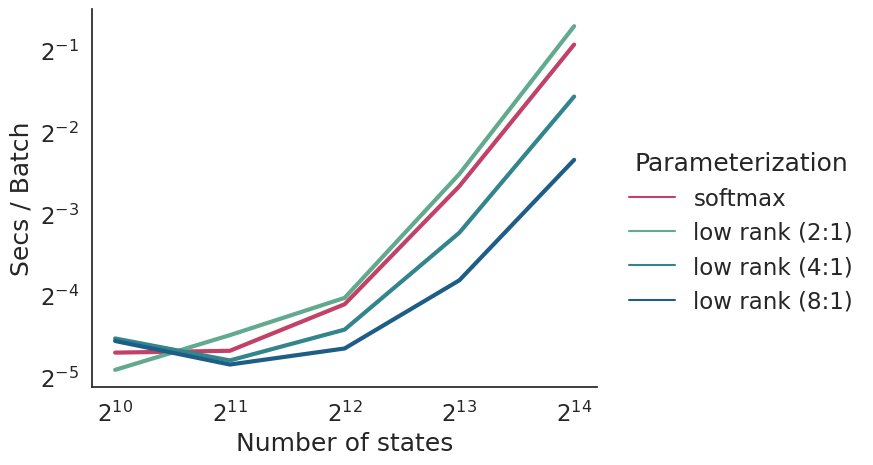
\includegraphics[height=4.5cm]{imgs/hmm/lhmm-states-features-speed-log.png}
\end{subfigure}
\caption{
\label{fig:hmm-ppl-features-dropout}
Validation perplexities on \textsc{Ptb} versus model scale, as well as speed in seconds per batch.
}
\end{figure}
Our main experimental result is that the low-rank models produce similar results as our baselines.
Fig.~\ref{fig:hmm-ppl-features-dropout} shows that perplexity improves as we increase the scale of the HMM, and
that the performance of our LHMM also improves at the same rate.
At small sizes, the low-rank constraints slightly hinder performance; however
once the size is large enough, i.e. larger than $2^{12}$, LHMMs with 8:1 state-to-rank ratios perform comparably. \footnote{
%One explanation is that while the rank constraint results in underfitting at smaller state sizes, at larger state sizes the transition matrix of the softmax HMMs is already lower rank due to implicit rank regularization \citep{gunasekar2017implicit,implicit-rank-reg,razin2020rank}, resulting in no loss of performance with a rank constraint in the corresponding LHMM.
See Appendix~\ref{sec:rank} for an analysis of the ranks of HMMs/LHMMs.}

Fig.~\ref{fig:hmm-ppl-features-dropout} also contains speed comparisons between HMMs and LHMMs.
A state-to-rank ratio of 8:1 matches the performance of softmax HMMs at larger state sizes and also gives an empirical speedup of more than 3x at $L = 2^{14}$.
As expected, we only see a speedup when the state-to-rank ratio exceeds 2:1, as we replaced the $O(L^2)$ operation with two $O(LN)$ ones. This implies that the low-rank constraint is most effective with scale, where we observe large computational gains at no cost in perplexity.



\begin{table}[!t]
\centering
\begin{minipage}[t]{0.4\textwidth}
\centering
\begin{tabular}{lrr}
\toprule
Model & Val & Test\\

\midrule
%AWD-LSTM-DOC & 54.1 & 52.4\\
AWD-LSTM & 60.0 & 57.3\\
VL-HMM & 128.6 & 119.5\\
HMM & 144.3 & 136.8\\
LHMM & 141.4 & 131.8\\
\bottomrule
\end{tabular}
\end{minipage}
\vspace{0em}
\hfill
\begin{minipage}[t]{0.55\textwidth}
\centering
\begin{tabular}{lrrr}
\toprule
Model & $L:N$ & Train & Val\\
\midrule
%AWD-LSTM-DOC & 54.1 & 52.4\\
HMM & -  & 95.9 & 144.3\\
LHMM & 8 & 97.5 & 141.4\\
LHMM+band & 8 & 101.1 & 143.8\\
LHMM & 16 & 110.6 & 146.3 \\
LHMM+band & 16 & 96.9 & 138.8\\
LHMM & 32 & 108.4 & 153.7 \\
LHMM+band & 32 & 110.7 & 145.0\\
\bottomrule
\end{tabular}
\end{minipage}
\vspace{0.5em}
\caption{\label{tbl:hmm}
Model perplexities on \textsc{Ptb}.
All HMM variants have $L=2^{14}$ states.
(Left): Validation and test perplexities.
The LHMM has a state-to-rank ratio $8:1$.
(Right): Further experiments with extending the low-rank structure of LHMMs with a banded transition structure.
}
%\vspace{-0.5cm}
\end{table}

%HMMs do not out-perform LSTM-based models on language modeling \citep{chiu2020scaling}, shown in Tbl.~\ref{tbl:hmm-ppl}.
% Comparison to LSTM and VL-HMM
%Additionally,

HMMs are outperformed by neural models,
and also by VL-HMMs \citep{chiu2020scaling} which offer similar modeling advantages to HMMs,
as shown in Tbl.~\ref{tbl:hmm}~(left).
This indicates that some aspects of performance are not strictly tied to scale. 
We posit this is due to the problem-specific block-sparse emission constraint in VL-HMMs. While 
very effective for language modeling,
the VL-HMM relies on a hard clustering of states for constraining emissions. 
This is difficult to apply to problems with richer emission models (as in music and video modeling).


\textbf{Hidden Markov Models for Music Modeling}
We next apply LHMMs on polyphonic music modeling. This has a max effective vocabulary size of $2^{88}$, as multiple notes may occur simultaneously. Unlike for language modeling, we use a factored Bernoulli emission model, modeling the presence of each note independently. Fig.~\ref{fig:music} (right) shows that HMMs are competitive with many of the models on these datasets, including LSTMs.
We find that LHMMs achieve performance slightly worse than but comparable to the unconstrained HMMs overall.
Fig.~\ref{fig:music} (left) shows that the distinction drops with more states. Both HMMs achieve low negative likelihoods (NLL) on the datasets with shorter sequences, Nottingham and JSB, but relatively poorer NLLs on the datasets with longer sequences (Muse and Piano).
%{\color{red} NEW}
%We hypothesize that the performance gap between HMM and LHMM, exacerbated by the datasets with longer sequences such as Piano and Muse, is due to the rank constraint at a relatively small state size.
%However, fitting larger HMMs and LHMMs does not lead to pronounced improvements in generalization.

\begin{figure}[t]
\centering
\begin{subfigure}{0.45\textwidth}
\centering
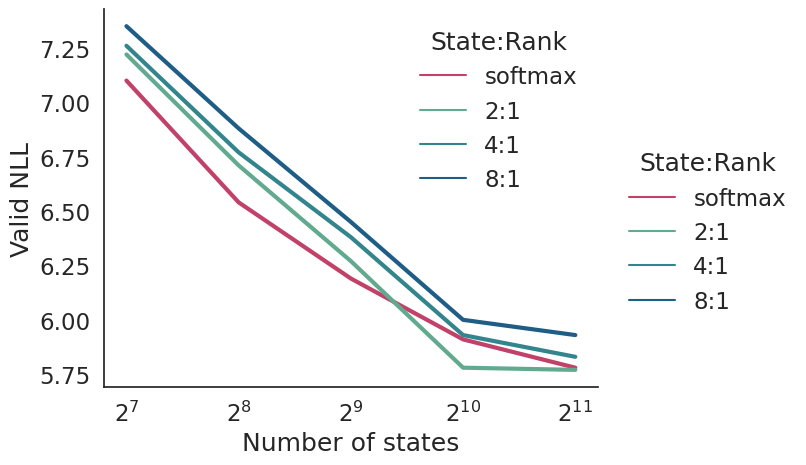
\includegraphics[height=4.5cm,trim={0 0 14.5em 0},clip]{imgs/hmm/music-states-features-dropout.png}
\end{subfigure}
\begin{subfigure}{0.50\textwidth}
\centering
\begin{tabular}{lrrrr}
\toprule
Model       & Nott & Piano & Muse & JSB \\
\midrule
%RNN      & 4.46       & 8.37        & 8.13       & 8.71          \\ 
%\midrule 
RNN-NADE & 2.31  & \textbf{7.05}        & \textbf{5.6}        & 5.19          \\
%\midrule
R-Transformer & \textbf{2.24} & 7.44 & 7.00 & 8.26 \\
LSTM  & 3.43 & 7.77   & 7.23 & 8.17     \\
%\midrule
LV-RNN    & 2.72       & 7.61        & 6.89       &\textbf{ 3.99}\\
SRNN     & 2.94       & 8.20         & 6.28       & 4.74          \\
\midrule
TSBN     & 3.67       & 7.89        & 6.81       & 7.48          \\
HMM &  2.43 & 8.51 & 7.34 & 5.74 \\
LHMM & 2.60 & 8.89 & 7.60 & 5.80 \\
\bottomrule
\end{tabular}
\end{subfigure}
\caption{\label{fig:music}
Polyphonic music negative log-likelihoods (NLL), measured in nats.
(Left): HMM and LHMM validation performance for various state sizes and state:rank ratios. 
(Right): Test-set NLLs for polyphonic music.
The HMM models have $\mcL=2^{11}$ states and the LHMM has rank $N=2^{9}$, a 4:1 state:rank ratio.}
\end{figure}

\begin{comment}
\begin{table}[!t]
\centering
\begin{tabular}{lrr}
\toprule
Model & Train & Val \\
\midrule
LHMM                         & 173 & 213\\
\quad + embedding normalization      & 174 & 215 \\
\quad + random $\phi_\textrm{pos}$ & 182 & 222\\
\quad + $\phi_{\exp}$              & 338 & 349\\
\quad + $\phi_\ReLU$               & 185 & 223\\
\bottomrule
\end{tabular}
\caption{\label{tbl:hmm-ablation}
Ablations for the embedding normalization and feature map on \textsc{Ptb} in a LHMM with a fixed number of states $|\mcL| = 256$ and features $n=256$.
We perform each ablation independently.
(RERUN AND MOVE TO APPENDIX)
}
\end{table}
\end{comment}

% PTB PARSING PCFG
\textbf{Context-Free Grammars}
For syntactic language modeling on \textsc{Ptb}, our low-rank PCFG (LPCFG) achieves similar performance to PCFGs, as shown in Table~\ref{tbl:cky} (left), with an improvement in computational complexity. The complexity of inference in PCFGs models is cubic in the number of nonterminals, so even models with $|\mcN|=30$ nonterminals are relatively
costly. Our approach achieves comparable results with $N=8$ features. As we scale up the number of nonterminals to $|\mcN| = 100$, LPCFG stays competitive with a lower computational complexity (since $N < |\mcN|$). These experiments also demonstrate the importance of scale in syntactic language models with more than 50 point gain in perplexity over a strong starting model.

\textbf{CFG Speed}
Once the model is large enough, i.e. $|\mathcal{N}|\ge 60$ nonterminals and
$|\mathcal{P}|\ge 120$ preterminals, the LPCFG is faster than PCFG,
as shown in Tbl.~\ref{tbl:cky} (left).
Note that the LPCFG is faster than the CFG even when the number of features
$N>\frac{|\mathcal{N}|}{2}$, in contrast to the HMM case where a speedup can only
be obtained when $N < L/2$.
This is due to the scoring matrix being rectangular:
Recall the low-rank matrix product
$\Psi\beta = U(V^\top\beta)$, where,
when specialized to PCFGs, the left-hand side takes time $O(L^{3})$
and the right-hand side takes $O(L^{2}N + LN)$.
For PCFGs, the term $V^\top\beta$ dominates the runtime.
This contrasts with HMMs, where both $V^\top\beta$ and the subsequent multiplication
by $U$ take the same amount of time, $O(LN)$.

% PCFG ablation studies moved to appendix
\textbf{Hidden Semi-Markov Models for Video Modeling} Table~\ref{tbl:cky} (right) shows the results of video modeling using HSMMs. In addition to using a different hypergraph, these experiments use a continuous Gaussian emission model. By removing the state constraints from tasks, our HSMM baselines get better video-level NLLs than that from \citet{fried2020learning} at the cost of more memory consumption. Due to GPU memory constraints, we can only train HSMMs up to $2^8$ states, but by using our low-rank parameterization, we can scale to up to $2^{10}$ states which yields an improved NLL. Absolute results could likely be improved with more states and by an improved emission parameterization for all models.

\textbf{Improving Rank Assumptions}
%(weakness of low rank HMM)
One potential limitation of all low-rank models is that they cannot learn high-rank structures with low $N$.
We began to see this issue at a ratio of 16:1 states to features for large HMMs.
To explore the effects of this limitation, we perform an additional experiment that combines low-rank features with a sparse component. Specifically we add an efficient high-rank sparse banded transition matrix. 
The full details are in Appendix~\ref{sec:banded}.
Tbl.~\ref{tbl:hmm} (right) shows that combination with the band structure allows for larger ratios than just the low-rank structure alone, while only adding another operation that costs $O(LN)$.

\begin{comment}
\begin{table}[!t]
\centering
\begin{minipage}[t]{0.47\textwidth}
\centering
\begin{tabular}{lllrrr}
\toprule
$|\mcN|$ & $|\mcP|$ & Model & $N$ &  PPL  \\
\midrule
30  & 60    & PCFG & - & 252.60 \\
%    &       & LPCFG & 4 & 255.42          \\
    &       & LPCFG & 8 &  247.02         \\
    &       & LPCFG & 16 & 250.59        \\
% 32>30, so maybe we shouldn't use this at all    &       & Kernel PCFG       & 32 &           \\
\midrule
60  & 120   & PCFG & - & 234.01\\ % this number is much higher than val, not sure why
    &       & LPCFG & 16& 217.24 \\
    &       & LPCFG & 32& 213.81 \\
\midrule
100 & 200   & PCFG & - &  191.08    \\
    &       & LPCFG & 32& 203.47 \\
    &       & LPCFG & 64& 194.25 \\
%    &       & Kernel PCFG       & 90& \\
\bottomrule
\end{tabular}

\end{minipage}
\vspace{0em}
\hfill
\begin{minipage}[t]{0.52\textwidth}
\centering
\begin{tabular}{lllrrr}
\toprule
Model & $L$ & $N$ & NLL \\
\midrule
\citet{fried2020learning} & $\le$151 & - & $1.432e5$\\ % 143,195.5214
\midrule
HSMM & $2^6$ & - & $1.428e5$ \\ % 142,764.6950
HSMM & $2^7$ & - & $1.427e5$ \\ % 142,676.1718
HSMM & $2^8$ & - & $1.426e5$ \\ % 142,560.6654
\midrule
%LHSMM & 128 & 32 & 142693.8505 \\
LHSMM & $2^7$ & $2^7$ & $1.427e5$ \\ % 142,705.0657
LHSMM & $2^8$ & $2^6$ & $1.426e5$ \\ % 142,560.1605
%LHSMM & 512 & 16 & 142502.4018 \
LHSMM & $2^9$ & $2^5$ & $1.424e5$ \\ % 142,405.2694
LHSMM & $2^{10}$ & $2^4$ & $1.423e5$ \\ % 142,291.8286
\bottomrule
\end{tabular}
\end{minipage}
\vspace{.5em}
\caption{\label{tbl:cky}
(Left): Test perplexities of PCFG models on \textsc{Ptb}. The complexity of PCFG is $O(T^3|\mcN|^3)$, whereas the complexity of LPCFG is $O(T^3 |\mcN|^2N)$. (Right): Negative log likelihoods (NLL) per video of HSMM models on \textsc{CrossTask}. We cannot train HSMMs beyond $2^8$ states due to GPU memory constraints, but we can train LHSMMs with up to $2^{10}$ states.
}
\end{table}
\end{comment}

\begin{table}[!t]
\centering
\begin{tabular} {lllrrrr}
\toprule
$|\mathcal{N}|$ & $|\mathcal{P}|$ & Model & $N$ &  PPL & Batch/s\\
\midrule
30  & 60    & PCFG & - & 252.60 & 4.37\\
    &       & LPCFG & 8 &  247.02    & 3.75\\
    &       & LPCFG & 16 & 250.59    & 3.74\\
\midrule
60  & 120   & PCFG & - & 234.01 & 2.99\\
    &       & LPCFG & 16& 217.24 & 3.55\\
    &       & LPCFG & 32& 213.81 & 3.35\\
\midrule
100 & 200   & PCFG & - &  191.08   & 0.98\\
    &       & LPCFG & 32& 203.47 & 1.56\\
    &       & LPCFG & 64& 194.25 & 1.24\\
\bottomrule
\end{tabular}
\vspace{0em}
\hfill
\begin{tabular} {lllrrrr}
\toprule
Model & $L$ & $N$ & NLL & Batch/s \\
\midrule
HSMM & $2^6$ & - & $1.428e5$ & 1.28 \\
HSMM & $2^7$ & - & $1.427e5$  & 0.45\\
HSMM & $2^8$ & - & $1.426e5$ & 0.13 \\
\midrule
LHSMM & $2^7$ & $2^7$ & $1.427e5$ & 0.24 \\
LHSMM & $2^8$ & $2^6$ & $1.426e5$ & 0.20 \\
LHSMM & $2^9$ & $2^5$ & $1.424e5$ & 0.18 \\
LHSMM & $2^{10}$ & $2^4$ & $1.423e5$ & 0.10 \\
\bottomrule
\end{tabular}
\vspace{.5em}
\caption{\label{tbl:cky}
(Left): Test perplexities and speeds for PCFG models on \textsc{Ptb}. The complexity of PCFG is $O(T^3|\mcN|^3)$, whereas the complexity of LPCFG is $O(T^3 |\mcN|^2N)$. Speeds are given in batches per second. (Right): Negative log likelihoods (NLL) per video and speeds for HSMM models on \textsc{CrossTask}. We cannot train HSMMs beyond $2^8$ states due to GPU memory constraints, but we can train LHSMMs with up to $2^{10}$ states. Speeds are given in batches per second.
}
\end{table}




\begin{comment}
\begin{table}[!htp]
\centering
\begin{tabular}{lllrr}
\toprule
\multicolumn{4}{c}{Kernel for $B\ C $} & \multirow{2}{*}{PPL}\\
\cmidrule{1-4}
$\mcN\times \mcN$ & $\mcN\times\mcP$  & $\mcP\times\mcN$ & $\mcP\times\mcP$ \\
\midrule
  Softmax & Softmax & Softmax & Softmax & 243.19\\
  Linear & Softmax & Softmax & Softmax & 242.72\\
  Linear & Linear & Linear & Softmax &  259.05 \\
  Linear & Linear & Linear & Linear & 278.60 \\
\bottomrule
\end{tabular}
\caption{\label{tbl:cky-ablation}
Ablation studies of PCFG. The perplexities are evaluated on the validation set of \textsc{Ptb}. Here we use $|\mcN|=30$, $|\mcP|=60$, and 16 features for linearlized kernel.
}
\end{table}
\end{comment}



\section{Related Work}

% Tractable latent variable models for sequences
%Speeding up and scaling latent variables for sequences has a long history.
Similar to our work, other approaches target matrix or tensor operations in inference, and impose structural model constraints to improve computational complexity.
Many of the works on HMMs in particular take advantage of the transition structure.
% Constraints for speeding up LVMs
The Dense-mostly-constant (DMC) HMM assigns a subset of learnable parameters per row of the transition matrix and sets the rest to a constant, leading to a sub-quadratic runtime \citep{dmc}.
%Our low-rank+band LHMM is a generalization of the DMC, where the banded LHMM has a fixed number of learnable entries around the transition diagonal and the rest of the entries left to a low-rank decomposition.
Other structures have also been explored, such as aligning the states of an HMM to underlying phenomena that allows inference to be sped up \citep{ffthmm,constrainedhmm}.
Additionally, other methods take advantage of emission structure in HMMs in order to scale, such as the Cloned HMM \citep{dedieu2019learning} and VL-HMM \citep{chiu2020scaling}.
Compared to these approaches, our method is more flexible and generic, since it can be applied in a non-application-specific manner, and even extended with high-rank components (such as banded structure).

Low-rank structure has been explored in both HMMs~\citep{rrhmm} and a generalization of PCFGs called weighted tree automata~\citep{rrpcfg}. The reduced-rank HMM~\citep{rrhmm} has at most 50 states, and relies on spectral methods for training.  The low-rank weighted tree automata~\citep{rrpcfg} also trains latent tree models via spectral methods. We extend the low-rank assumption to neural parameterizations, which have been shown to be effective for generalization \citep{kim2019cpcfg,chiu2020scaling}, and directly optimize the evidence via gradient descent.

Concurrent work in unsupervised parsing uses a tensor decomposition to scale PCFGs to large state spaces \citep{yang2021pcfgs}. Our low-rank decomposition of the flattened head-tail scoring matrix is more general, resulting in worse scaling for the PCFG setting but with wider applicability, as shown by experiments with HMMs.% and HSMMs.

% is this really necessary? Yes, I think
Kernels have been used in non-parametric belief propagation for graphical models~\citep{song2011kernelbp,song2010kernelhmm,song2011kerneltree}, with the goal of performing approximate inference in complicated, non-conjugate models.
We utilize kernels in the context of standard models, then scale them to massive sizes.


%Since we turn to kernels to improve computational efficiency by introducing constraints, our work contrasts with much of the focus ernels to increase model flexibility~\citep{svm}.

%\footnote{This approach is related to kernel belief propagation,however the underlying model assumptions are different~\citep{song2011kernelbp}.Kernel belief propagation uses cross-covariance operatorsto nonparametrically estimate dependencies between random variables, whereas we assume both immediate access to conditional distributions and even impose further constraints on those distributions in order to improve computational efficiency.}

%Separately, work on linear time and space attention has made tremendous progress, coming close to \citep{shen2018linearattn,katharopoulos2020lineartransformer,wang2020linformer} or matching \citep{choromanski2020performer,peng2021rfa} the performance of regular softmax attention, which takes time quadratic in the length of a sequence. This work builds upon prior work in viewing attention through the lens of a kernel \citep{tsai2019kernelattn}, as well as kernel-based approximations for sampled softmax \citep{blanc2018sampledsoftmax,rawat2019sampledsoftmax}. This line of work also expresses attention as a matrix-vector product, then uses a low-rank decomposition to speed up said product. We draw our kernel parameterizations from \citet{choromanski2020performer}, and extend their application to the structured prediction setting.

%Kernel embeddings of graphical models have been applied to a variety of settings: HMMs \citep{song2010kernelhmm} and latent trees \citep{song2011kerneltree}. While kernelized representations are used in both kernel belief propagation (KBP) \citep{song2011kernelbp} as well as our kernelized inference, KBP uses kernel representations to perform approximate inference in intractable models. In contrast, we introduce constraints in relatively simple models in order to scale to large state spaces, while remaining in a simple model family. Additionally, we capitalize on modern parallel hardware in order to scale to much larger models than previously considered.


\section{Conclusion}

This work improves the scaling of structured models by establishing the effectiveness of low-rank constraints for hypergraph models. We show that viewing a key step of inference in structured models as a matrix-vector product, in combination with a low-rank constraint on relevant parameters, allows for an immediate speedup. 
Low-rank inference allows us to obtain a reduction in the asymptotic complexity of marginalization at the cost of 
a constrained model. 
Our approach applies to a wide class of models, including HMMs, HSMMs, and PCFGs. Through our experiments on language, video, and polyphonic music modeling, we demonstrate an effective approach for overcoming the practical difficulty of applying low-rank constraints in high dimensional, structured spaces by targeting and constraining model components that bottleneck computation. Future work includes exploration of other structural constraints for speeding up matrix-vector products~\citep{kaleidoscope} performed in inference, as well as application to models where exact inference is intractable.

\begin{ack}
We thank Nikita Kitaev for the discussion that sparked this project.
We thank Sam Wiseman and the anonymous reviewers for helpful feedback.
\end{ack}



\bibliography{bib}
\bibliographystyle{plainnat}

%%%%%%%%%%%%%%%%%%%%%%%%%%%%%%%%%%%%%%%%%%%%%%%%%%%%%%%%%%%%
\begin{comment}
\section*{Checklist}

\begin{enumerate}

\item For all authors...
\begin{enumerate}
  \item Do the main claims made in the abstract and introduction accurately reflect the paper's contributions and scope?
    \answerYes{}, we demonstrate a 3x speedup in large HMMs via kernelization in Fig.~\ref{fig:hmm-ppl-features-dropout}.
  \item Did you describe the limitations of your work?
    \answerYes{}, we mention the limitation of the low-rank constraint in Section~\ref{sec:results}.
  \item Did you discuss any potential negative societal impacts of your work?
    \answerYes{}, see Appendix~\ref{sec:impact}.
  \item Have you read the ethics review guidelines and ensured that your paper conforms to them?
    \answerYes{}
\end{enumerate}

\item If you are including theoretical results...
\begin{enumerate}
  \item Did you state the full set of assumptions of all theoretical results?
    \answerNA{}{}
	\item Did you include complete proofs of all theoretical results?
    \answerNA{}
\end{enumerate}

\item If you ran experiments...
\begin{enumerate}
  \item Did you include the code, data, and instructions needed to reproduce the main experimental results (either in the supplemental material or as a URL)?
    \answerYes{}, we will include code in the supplemental material.
  \item Did you specify all the training details (e.g., data splits, hyperparameters, how they were chosen)?
    \answerYes{}, see Section~\ref{sec:experiments} and Appendix~\ref{sec:data} and \ref{sec:opt}.
	\item Did you report error bars (e.g., with respect to the random seed after running experiments multiple times)?
    \answerNo{}, we will include error bars in future revisions.
	\item Did you include the total amount of compute and the type of resources used (e.g., type of GPUs, internal cluster, or cloud provider)?
    \answerYes{}, see Appendix~\ref{sec:opt}.
\end{enumerate}

\item If you are using existing assets (e.g., code, data, models) or curating/releasing new assets...
\begin{enumerate}
  \item If your work uses existing assets, did you cite the creators?
    \answerYes{} we cite the datasets and models.
  \item Did you mention the license of the assets?
    \answerYes{}, we include the license in the code with the supplemental material.
  \item Did you include any new assets either in the supplemental material or as a URL?
    \answerYes{}, we include code in the supplemental material.
  \item Did you discuss whether and how consent was obtained from people whose data you're using/curating?
    \answerNo{}, the data for the Penn Treebank and polyphonic music are publicly available.
  \item Did you discuss whether the data you are using/curating contains personally identifiable information or offensive content?
    \answerNo{}, we are not aware of the Penn Treebank containing personally identifiable information or offensive content, and the music datasets are not applicable.
\end{enumerate}

\item If you used crowdsourcing or conducted research with human subjects...
\begin{enumerate}
  \item Did you include the full text of instructions given to participants and screenshots, if applicable?
    \answerNA{}
  \item Did you describe any potential participant risks, with links to Institutional Review Board (IRB) approvals, if applicable?
    \answerNA{}
  \item Did you include the estimated hourly wage paid to participants and the total amount spent on participant compensation?
    \answerNA{}
\end{enumerate}

\end{enumerate}
\end{comment}
%%%%%%%%%%%%%%%%%%%%%%%%%%%%%%%%%%%%%%%%%%%%%%%%%%%%%%%%%%%%
\newpage

\appendix

%\section{Appendix}
\section{\label{sec:expressivity}Expressivity of Low-Rank Models}
We focus on the simplest case of HMMs for an analysis of expressivity.
In the case of Gaussian emissions, \citet{rrhmm} show that for a single timestep a model with more states but low rank is more expressive than a model with fewer states. {\color{red}<- Double check this}
In the case of discrete emissions, however, the emission distribution for a single timestep is not more expressive. Instead, we show that there exist joint marginal distributions of $x$ over multiple timesteps that are not captured by models with fewer states.
{\color{red}Copy paste proof here}

even in the discrete case, an HMM with a transition matrix of rank N cannot always be converted to an equivalent HMM with N states: while a rank-N HMM can be converted to an N-dimensional PSR (Predictive State Representations), PSRs are a larger class than HMMs (the states of PSRs are N-dimensional continuous vectors). In fact, Siddiqi et al 2010 [rrhmm] mentioned “So, rank-k RR-HMMs (which can have m >> k states) can model sets of predictive distributions which k-state HMMs cannot.” (Section 2.1, last paragraph, note that this statement does not specify whether it's discrete or continuous).

We can use a concrete example to show that there are distributions that rank-N HMMs can model but N-state HMMs cannot: let sequence length $T=2$, rank $N=2$, observations $x_t\\in\\{0, 1, 2\\}$.

1. Specification of a rank-2 HMM with 3 states ($z_t\in \{0,1,2\}$):

transition probabilities (rows $z_t$, columns $z_{t+1}$):
$$
P(z_{t+1} |z_{t})
= \begin{bmatrix}
    \frac{1}{3} & \frac{1}{3} & \frac{1}{3} \\
    0 & 1 & 0 \\
    \frac{1}{2} & 0 & \frac{1}{2}
\end{bmatrix}
=  \begin{bmatrix}
    \frac{1}{3} & \frac{2}{3} \\
    1 & 0 \\
    0 & 1
\end{bmatrix}
\begin{bmatrix}
    0 & 1 & 0 \\
    \frac{1}{2} & 0 & \frac{1}{2}
\end{bmatrix} = UV^T
$$

emission probabilities (rows $z_t$, columns $x_t$):
$$P(x_t|z_t) = \begin{bmatrix}1 &0 & 0 \\ 0 & 1 & 0 \\ 0 & 0 &1\end{bmatrix}$$

initial auxiliary state: $z_0 = 0$,
such that the distribution of the first state
$$P(z_1) =  \begin{bmatrix}\frac{1}{3} & \frac{1}{3} & \frac{1}{3}\end{bmatrix}$$

Then the marginal distribution (row $x_1$, column $x_2$):
$$
P(x_1, x_2) = \begin{bmatrix}
    \frac{1}{9} & \frac{1}{9} & \frac{1}{9} \\
    0 & \frac{1}{3} & 0 \\
    \frac{1}{6} & 0 & \frac{1}{6}
\end{bmatrix}.
$$

We will show in the following that this marginal is not achievable under a 2-state HMM.
The intuition is that the second row ($P(x_2|x_1=1)= \begin{bmatrix}0& 1 & 0\end{bmatrix}$)
would need one state $z_2=a$ to model
(and this state will only emit $x_t=1$, and the third row
($P(x_2|x_1=2)= \begin{bmatrix}0.5& 0 & 0.5\end{bmatrix}$)
would need the other state $z_2=b\ne a$ to model (since $a$ cannot emit $x_t=0$).
We know that $z_1=b$ for $x_1=2$ since $z_1=a$ can only emit $x_1=1$,
then the last row also tells us that $z_1=b$ cannot transition to $z_2=a$,
since otherwise $P(x_2=1|x_1=2)$ would be nonzero (because $z_2=a$ can emit $x_2=1$).
Now for the first row ($P(x_2|x_1=0)$),
the state $z_1$ must be $b$ since $z_1=a$ cannot emit $x_1=0$,
so $z_2$ must also be $b$ because $b$ cannot transit to $a$.
Then $P(x_2=1|x_1=0)$ would also be 0 since $b$ cannot emit 1,
contradicting the given marginals.

Below provides a more rigorous argument.

There does not exist any 2-state HMM with the above marginal distribution.
To prove this, we will first show that there is only one valid emission distribution
in a 2-state HMM, and then derive a contradiction when we look at transitions.

We will use the equations
$P(x_1, x_2) = \sum_{z_2}\left[\sum_{z_1}P(z_1)P(x_1|z_1)P(z_2|z_1)\right]P(x_2|z_2)$.
We denote $\sum_{z_1}P(z_1)P(x_1|z_1)P(z_2|z_1)$ as $f(x_1,z_2)$,
then we can write those equations in the matrix form:

$$
\begin{bmatrix} f(0, 0) & f(0, 1) \\ f(1, 0) & f(1, 1) \\ f(2, 0) & f(2, 1) \end{bmatrix}
\begin{bmatrix} P(x_2|z_2=0) \\ P(x_2|z_2=1) \end{bmatrix}
= P(x_1, x_2)
=  \begin{bmatrix}
    \frac{1}{9} & \frac{1}{9} & \frac{1}{9} \\
    0 & \frac{1}{3} & 0 \\
    \frac{1}{6} & 0 & \frac{1}{6}
\end{bmatrix}
$$

Looking at the second row of this equation: $f(1,0) P(x_2|z_2=0) + f(1,1)P(x_2|z_2=1)= \begin{bmatrix}0 & \frac{1}{3} & 0 \end{bmatrix}$, $f(1,0)$ and $f(1,1)$ can't be both 0 since otherwise the result would be a zero vector. Without loss of generality, assume $f(1,0)\ne 0$, then $P(x_2=0|z_2=0)=P(x_2=2|z_2=0)=0$, since all terms are non-negative and if any of them is greater than
0, then the result would be greater than 0 at the corresponding position. Therefore, $P(x_2|z_2=0)=\begin{bmatrix}0 & 1& 0 \end{bmatrix}$.

Now let's look at the last row of the equation: $f(2,0) P(x_2|z_2=0) + f(2,1)P(x_2|z_2=1)= \begin{bmatrix} \frac{1}{6} &0 &  \frac{1}{6} \end{bmatrix}=P(x_2|x_1=2)$. Since $P(x_2|z_2=0)=\begin{bmatrix}0 & 1& 0 \end{bmatrix}$, $f(2,0)$ must be 0, otherwise the result would have a non-zero $P(x_2=1|x_1=2)$. Therefore, $f(2,1)P(x_2|z_2=1)= \begin{bmatrix} \frac{1}{6} &0 &  \frac{1}{6} \end{bmatrix}$, hence $P(x_2|z_2=1)= \begin{bmatrix} \frac{1}{2} &0 &  \frac{1}{2} \end{bmatrix}$.

Putting the above two paragraphs together, we have the full emission matrix now: $P(x_t|z_t)=\begin{bmatrix}0 & 1& 0\\  \frac{1}{2} &0 &  \frac{1}{2}  \end{bmatrix}$.

Using this emission matrix, we can find deterministic posterior mappings from observed variables $x_1$ to latent variables $z_1$. First, since $P(x_1=1|z_1=1)=0$ , we have $P(z_1=1|x_1=1)=0$ using Bayes’ rule, so $P(z_1=0|x_1=1)=1$. Similarly, we can prove that $P(z_1=1|x_1=0)=1$ and $P(z_1=1|x_1=2)=1$.

Now we can find a contradiction when we consider transitions from $z_1$ to $z_2$: first we will prove that $z_1=1$ cannot transit to $z_2=0$ and can only transit to $z_2=1$:  $P(x_2=1|x_1=2)\ge P(x_2=1, z_2=0, z_1=1|x_1=2) = P(x_2=1|z_2=0)P(z_2=0|z_1=1)P(z_1=1|x_1=2)$, substituting  $P(z_1=1|x_1=2)=1$ and $P(x_2=1|z_2=0)=1$ into this inequality, we have $P(x_2=1|x_1=2)\ge P(z_2=0|z_1=1)$. Since $P(x_2=1|x_1=2)=0$, we have $P(z_2=0|z_1=1)=0$. Then we will show that $P(x_2=1|x_1=0)$ must be 0 since $z_1|x_1=0$ has to be 1 and it can only transit to $z_2=1$ which cannot emit $x_2=1$:  $P(x_2=1|x_1=0) = \sum_{z_1, z_2}P(x_2=1, z_1, z_2|x_1=0) =  \sum_{z_1, z_2}P(x_2=1 | z_2)P(z_2|z_1) P(z_1|x_1=0)$. Since $P(z_1=0|x_1=0)=0$, $P(x_2=1|x_1=0) =\sum_{z_2} P(x_2=1|z_2)P(z_2|z_1=1)P(z_1=1|x_1=0)$. Since $P(z_2=0|z_1=1)=0$, this sum can further reduce to $P(x_2=1|x_1=0) =P(x_2=1|z_2=1)P(z_2=1|z_1=1)P(z_1=1|x_1=0)$. Using the emission matrix, $P(x_2=1|z_2=1)=0$, so $P(x_2=1|x_1=0) =0$, which contradicts the desired marginal $P(x_2=1|x_1=0) =\frac{1}{3}$. Therefore, we have completed the proof that it is impossible to use an HMM with 2 states to get the same marginal distribution.


\section{\label{sec:low-rank-marg}Low-Rank Hypergraph Marginalization for HMMs and PCFGs}
We provide the low-rank hypergraph marginalization algorithms for HMMs and PCFGs in
Alg.~\ref{alg:lr-marg-hmm-pcfg},
with loops over labels $z$ (and products of labels) and feature dimensions $n$ left implicit for brevity.
We also assume that the label sets for PCFG are uniform for brevity -- in practice,
this can easily be relaxed (this was not assumed in Alg.~\ref{fig:marg-hmm-pcfg}).
We show how the normalizing constants $c$ are explicitly computed using the unnormalized
low-rank factors in each algorithm.

\begin{algorithm}[H]
\caption{Low-rank hypergraph marginalization for HMMs and PCFGs}
\label{alg:lr-marg-hmm-pcfg}
\begin{minipage}[t]{0.45\textwidth}
%\small
\begin{algorithmic}
\STATE {[\textit{HMM - Backward}]}
\STATE $[\tilde{V}]_{z,n} = [\phi(g(z))]_n$
\STATE $[\tilde{U}]_{z,n} = [\phi(f(z))]_n$
\STATE $[c]_z = [\tilde{U}\tilde{V}^\top\mathbf{1}]_z$
\FOR {$t \leftarrow (t+1)$ in right-to-left order}
\STATE $[\beta_{t+1}]_{z_{t+1}} = [\alpha_{t+1}]_{z_{t+1}}$
\STATE $[V_t]_{z_{t+1},n} = [\tilde{V}]_{z_{t+1},n}$
\STATE $[U_t]_{z_t,n} = p(x_t \mid z_t)[c]_{z_{t}}[\tilde{U}]_{z_t,n}$
\STATE $\alpha_t \stackrel{+}{\gets} U_t(V_t^\top\beta_{t+1})$
\ENDFOR
\STATE \textbf{return} $\alpha_0^\top \mathbf{1}$
\end{algorithmic}
\end{minipage}
\vspace{0pt}
\begin{minipage}[t]{0.50\textwidth}
%\small
\begin{algorithmic} 
\STATE {[\textit{PCFG - CKY}]}
\STATE $[\tilde{V}]_{z_1,z_2,n} = [\phi(g(z_1,z_2))]_n$
\STATE $[\tilde{U}]_{z_u,n} = [\phi(f(z_u))]_n$
\STATE $[c]_{z_u} = [UV^\top\mathbf{1}]_{z_u}$
\FOR {$(i,k) \leftarrow (i,j), (j,k)$ in span-size order}
\STATE $[\beta_{i,j,k}]_{(z_1,z_2)} = [\alpha_{i,j}]_{z_1}[\alpha_{j,k}]_{z_2}$
\STATE $[V_{i,j,k}]_{z_1,z_2,n} = [\tilde{V}]_{z_1,z_2,n}$
\STATE $[U_{i,j,k}]_{z_u,n} = [c]_{z_u}[\tilde{U}]_{z_u,n}$
\STATE $\alpha_{i,k} \stackrel{+}{\gets} U_{i,j,k}(V_{i,j,k}^\top\beta_{i,j,k})$
\ENDFOR
\STATE \textbf{return} $\alpha_{1,T}^\top \mathbf{1}$
\end{algorithmic}
\end{minipage}
\end{algorithm}

\section{Extension of the Low-Rank Constraint to Other Semirings}
Enforcing low-rank constraints in the scoring matrices $\Psi_e$
leads to a speedup for the key step in the hypergraph marginalization algorithm:
\begin{equation}
    \Psi_e\beta_v =  \left(U_e V_e^\top\right) \beta_v =  U_e\left(V_e^\top\beta_v\right),
\end{equation}
where $[\beta_v]_{z_1,z_2} = [\alpha_1]_{z_1}[\alpha_2]_{z_2}$.
While the low-rank constraint allows for speedups in both the log and probability semirings
used for marginal inference,
the low-rank constraint does not result in speedups in the tropical semiring,
used for MAP inference.
To see this, we first review the low-rank speedup in scalar form.
The key matrix-vector product step of marginal inference in scalar form is given by
\begin{align*}
\sum_{z_1,z_2} [\Psi_e]_{z_u,(z_1,z_2)}[\beta]_{z_1,z_2}
&= \sum_{z_1,z_2} \sum_n [U_e]_{z_u,n}[V_e]_{(z_1,z_2),n}[\beta]_{z_1,z_2}\\
&= \sum_n \sum_{z_1,z_2} [U_e]_{z_u,n}[V_e]_{(z_1,z_2),n}[\beta]_{z_1,z_2}\\
&= \sum_n [U_e]_{z_u,n}\sum_{z_1,z_2} [V_e]_{(z_1,z_2),n}[\beta]_{z_1,z_2},
\end{align*}
which must be computed for each $z_u$.
The first line takes $O(\mcL^{|e|+1})$ computation,
while the last line takes $O(\mcL^{|e|}N)$ computation.
The speedup comes rearranging the sum over $(z_1,z_2)$ and $n$,
then pulling out the $U_e$ factor, thanks to the distributive
propery of multiplication.
When performing MAP inference instead of marginal inference,
we take a max over $(z_1,z_2)$ instead of a sum.
Unfortunately, in the case of the max-times semiring used for MAP inference,
we cannot rearrange max and sum,
preventing low-rank models from obtaining a speedup:
\begin{align*}
\max_{z_1,z_2} [\Psi_e]_{z_u,(z_1,z_2)}[\beta]_{z_1,z_2}
&= \max_{z_1,z_2} \sum_n [U_e]_{z_u,n}[V_e]_{(z_1,z_2),n}[\beta]_{z_1,z_2}\\
&\ne \sum_n \max_{z_1,z_2} [U_e]_{z_u,n}[V_e]_{(z_1,z_2),n}[\beta]_{z_1,z_2}.
\end{align*}

\section{\label{sec:data}Data Details}
For language modeling on \textsc{Penn Treebank} (\textsc{Ptb}) \citep{ptb}
we use the preprocessing from \citet{mikolov-2011},
which lowercases all words and substitutes OOV words with UNKs. 
The dataset consists of 929k training words, 73k validation words, and 82k test words, with a vocabulary of size 10k.
Words outside of the vocabulary are mapped to the UNK token.
We insert EOS tokens after each sentence, and model each sentence, including the EOS token, independently.

The four polyphonic music datasets, Nottingham (Nott), Piano, MuseData (Muse), and JSB chorales (JSB), are used with the same splits as \citet{polyphonic}. The data is obtained via the following \href{https://github.com/pyro-ppl/pyro/blob/d7687ae0f738bd81a792dabbb18a53c0fce73765/pyro/contrib/examples/polyphonic_data_loader.py}{script}. Each timestep consists of an 88-dimensional binary vector indicating whether a particular note is played. Since multiple notes may be played at the same time, the effective vocabulary size is extremely large. The dataset lengths are given in Table~\ref{tbl:music-data}.



\begin{table}[t]
    \centering
    \begin{tabular}{lrrrr}
        \toprule
                & & \multicolumn{3}{c}{Total Length}\\
                \cmidrule{3-5}
        Dataset & Avg Len &  Train & Valid & Text \\
        \midrule
        Nott & 254.4 & 176,551 & 45,513  & 44,463 \\
        Piano& 872.5 & 75,911 & 8,540& 19,036 \\
        Muse & 467.9 &  245,202 & 82,755 & 64,339 \\
        JSB & 60.3 & 64,339 & 4,602 & 4,725\\
        \bottomrule
    \end{tabular}
    \caption{\label{tbl:music-data}The lengths for the four polyphonic music datasets. The average length of an example in the training split for each dataset is given.}
\end{table}

In experiments with PCFGs for language modeling, we also use \textsc{Ptb}, but with the splits and preprocessing used in unsupervised constituency parsing \citep{shen2018prpn,shen2018ordered,kim2019cpcfg}. This preprocessing discards punctuation, lowercases all tokens, and uses the 10k most frequent words as the vocabulary.
The splits are as follows: sections 2-21 for training, 22 for validation, 23 for test. Performance is evaluated using perplexity.

In experiments with HSMMs for video modeling, we use the \textit{primary} section of the \textsc{CrossTask} dataset \citep{zhukov2019cross}, consisting of about 2.7k instructional videos from 18 different tasks such as ``Make Banana Ice Cream'' or ``Change a Tire''. We use the preprocessing from \citet{fried2020learning}, where pretrained convolutional neural networks are first applied to extract continuous image and audio features for each frame, followed by PCA to project features to 300 dimensions.\footnote{\url{https://github.com/dpfried/action-segmentation}} We set aside 10\% of the training videos for validation.
\section{\label{sec:hsmm}Generative Process of HSMM} 

We use an HSMM to model the generative process of the sequence of continuous features for each video. The HSMM defines the following generative process: first, we sample a sequence of discrete latent states $z=(z_1, \cdots, z_K)$ with a first-order Markov model.
%A notable difference from HMMs is that we sample variable-length sequences as opposed to a fixed length sequence, by introducing a special end-of-sequence state. 
Next, we sample the length of observations under each state from a Poisson distribution $l_k\sim \text{Poisson}(\lambda_{z_k})$ truncated at max length $M$. The joint distribution is defined as
\begin{equation}
 \label{eqn:hsmmjoint}
     p(x, z, l) = \prod_{k=1}^K p(z_k \mid z_{k-1}) \ p(l_k \mid z_k)\prod_{i=l_1+\cdots+l_{k-1}}^{l_1+\cdots+l_k} p(x_i\mid z_k),
 \end{equation}
where the sequence length $T$ can be computed as $T=\sum_{k=1}^K l_k$. In this work, we only consider modeling continuous $x_t$, so we use a Gaussian distribution for $p(x_i\mid z_k)$.

To compute $p(x)$, we can marginalize $l, z$ using dynamic programming similar to HMMs, except that we have an additional factor of $M$: the overall complexity is $O(T\times M \times L^2)$ (ignoring the emission part since they are usually not the bottleneck). We refer to \citet{yu2010hidden} for more details.

\section{\label{sec:mlp-param}Full Parameterization of HMMs, PCFGs, and HSMMs}
In this section, we present more details on the parameterizations of the HMM, PCFG, and HSMM.
The main detail is where and how are neural networks used to parameterize state representations.

For low-rank HMMs (LHMMs) we  use the following mixed kernel parameterization that specifically targets the state-state bottleneck:
\begin{equation}
\begin{aligned}
p(z_1 \mid z_0) &\propto K(f_1(\bu_{z_0}), \bv_{z_1}), &
p(z_t \mid z_{t-1}) &\propto K(\bu_{z_{t-1}}, \bv_{z_t}), &
p(x_t \mid z_t) &\propto K_\SM(\bu_{z_t}, f_2(\bv_{x_t})),
\end{aligned}
\end{equation}
where $\bu_{z}$ is the embedding of $z$ when $z$ is used as head, $\bv_{z}$ its embedding when used as tail, and $f_1, f_2$ are MLPs with two residual layers. The efficiently linearizable kernel $K$ uses the feature map $\phi(x) = \exp(Wx)$. 

The PCFG uses a similar mixed parameterization. These probabilities correspond to start ($S\to A$), preterminal ($T\to x$), and standard productions ($A\to B\ C$) respectively.
\begin{equation}
\label{eqn:pcfgparam}
\begin{aligned}
p(z_{1,N} \mid S ) &\propto K_\SM(f_1(\bu_{S}), \bu_{z_{1,N}}),\\
p(x_i \mid z_i) &\propto K_\SM(\bu_{z_i}, f_2(\bv_{x_i})),\\
p( z_{i,j}, z_{j,k} \mid z_{i,k}) &\propto \begin{cases}
  K_\SM(\bu_{z_{i,k}}, \bv_{z_{i,j}\ z_{j,k}}) & \substack{i+1 = j \lor \\j+1=k} \\ 
 K(\bu_{z_{i,k}}', \bv_{z_{i,j}\ z_{j,k}}) &\text{o.w.} \\
\end{cases}\\
\end{aligned}
\end{equation}
where $\bu_{z}$/$\bu_z'$ is the embedding of $z$ when $z$ is used as head,$\bv_{x}$/$\bv_{z_1, z_2}$ is the embedding of $x$/$(z_1, z_2)$ when they are used as tail, and $f_1, f_2$ are MLPs with two residual layers as in \citet{kim2019cpcfg}. The efficiently linearizable kernel $K$ uses the feature map $\phi(x) = \exp(Wx - \|x\|_2^2/2)$.

For both HMMs and neural PCFG models, we use the same parameterization of the MLPs $f_1$ and $f_2$ as \citet{kim2019cpcfg}:
\begin{equation}
\label{eqn:res}
\begin{aligned}
f_i(x) &= g_{i,1}(g_{i,2}(W_i x)),\\
g_{i,j}(y) &= \ReLU(U_{i,j} \ReLU(V_{i,j} y)) + y,
\end{aligned}
\end{equation}
with $i,j \in \set{1,2}$, and
$W_i,V_{i,j},U_{i,j} \in \R^{D \times D}$. 


For HSMMs, the baseline ({HSMM} in Table~\ref{tbl:cky}) follows the fully unsupervised setting in \citet{fried2020learning} except that we don't apply any state constraints from the prior knowledge of each task.\footnote{We got rid of those constraints to allow for changing the total number of states, since otherwise we can't make any changes under a predefined state space.} The model maintains a log transition probability lookup table for $p(z_k \mid z_{k-1})$, a lookup table for the log of the parameters of the Poisson distribution $\lambda_{z_k}$. We maintain a mean and a diagonal covariance matrix for the Gaussian distribution $p(x_i\mid z_k)$ for each $z_k$. For low-rank HSMMs (LHSMMs), we use the same linearizable kernel parameterization for $p(z_k \mid z_{k-1})$ as in HMMs:
\begin{equation}
    p(z_k \mid z_{k-1}) \propto K(\bu_{z_{t-1}}, \bv_{z_t}),
\end{equation}
where $\bu_{z}$ is the embedding of $z$ when $z$ is used as head, $\bv_{z}$ its embedding when used as tail.  The linearizable kernel $K$ uses the feature map $\phi(x) = \exp(Wx)$. The emission parameterization is the same as in baseline HSMMs.

\section{\label{sec:opt}Initialization and Optimization Hyperparameters}
We initialize the parameters of feature maps in linearizable kernels using orthogonal feature projections \citep{choromanski2020performer}, and update it alongside the model parameters during training.

HMM parameters are initialized with the Xavier initialization \citep{glorot2010understanding}.\footnote{
For banded experiments, we initialize the band parameters by additionally adding 30 to each element.
Without this the band scores were too small compared to the kernel scores, and were ignored by the model.
}
We use the AdamW \citep{adamw} optimizer with a learning rate of $0.001$, $\beta_1=0.9,\beta_2=0.999$, weight decay 0.01, and a max grad norm of 5.
We use a state dropout rate of 0.1, and additionally have a dropout rate of 0.1 on the feature space of LHMMs.
We train for 30 epochs with a max batch size of 256 tokens, and anneal the learning rate by dividing by 4 if the validation perplexity fails to improve after 4 evaluations. Evaluations are performed 4 times per epoch.
The sentences, which we model independently from one another, are shuffled after every epoch.
Batches of sentences are drawn from buckets containing sentences of similar lengths to minimize padding. 

For the polyphonic music datasets, we use the same hyperparameters as the language modeling experiments, except a state dropout rate of 0.5 for JSB and Nottingham, 0.1 for Muse and Piano. We did not use feature space dropout in the LHMMs on the music datasets. For Nottingham and JSB, sentences were batched in length buckets, the same as language modeling. Due to memory constraints, Muse and Piano were processed using BPTT with a batch size of 8 for Muse and 2 for Piano, and a BPTT length of 128. We use $D=256$ for all embeddings and MLPs on all datasets, except Piano, which due to its small size required $D=64$ dimensional embeddings and MLPs. % i think this is only for hmms so moved it up here

For PCFGs, parameters are initialized with the Xavier uniform initialization \citep{glorot2010understanding}.
We follow the experiment setting in \citet{kim2019cpcfg} and use the Adam \citep{kingma2017adam} optimizer with $\beta_1=0.75,\beta_2=0.999$, a max grad norm of 3, and we tune the learning rate from $\{0.001, 0.002\}$ using validation perplexity. We train for 15 epochs with a batch size of 4. The learning rate is not annealed over training, but a curriculum learning approach is applied where only sentences of at most length 30 are considered in the first epoch. In each of the following epochs, the longest length of sentences considered is increased by 1.

For HSMMs, we use the same initialization and optimization hyperparameters as \citet{fried2020learning}: The Gaussian means and covariances are initialized with empirical means and covariances (the Gaussian parameters for all states are initialized the same way and they only diverge through training). The transition matrix is initialized to be uniform distribution for baseline HSMMs, and the transition embeddings are initialized using the Xavier initialization for LHSMMs. The log of Poisson parameters are initialized to be 0. We train all models for 4 epochs using the Adam optimizer with initial learning rate of 5e-3, and we reduce the learning rate 80\% when log likelihood doesn't improve over the previous epoch. We clamp the learning rate to be at least 1e-4. We use a batch size of 5 following \citet{fried2020learning}, simulated by accumulating gradients under batch size 1 in order to scale up the number of states as much as we can. Gradient norms are clipped to be at most 10 before updating. Training take 1-2 days depending on the number of states and whether a linearizable kernel is used.


We use the following hardware for our experiments: for HMMs we run experiments on 8 Titan RTX GPUs with 24G of memory on an internal cluster. For PCFGs and HSMMs we run experiments on 1 Nvidia V100 GPU with 32G of memory on an internal cluster.

\section{HMM Rank Analysis}
\label{sec:rank}

Table~\ref{tbl:hmm-rank} contains the empirical ranks of trained HMMs and LHMMs, estimated by counting the number of singular values greater than 1e-5. Note that the feature dimension $N$ is the maximum attainable rank for the transition matrix of an LHMM. Although LHMMs often manage to achieve the same validation perplexity as HMMs at relatively small $N$, the ranks of the transition matrices are much lower than both their HMM counterparts as well as $N$.
At larger state sizes, the ranks of learned matrices are almost half of their max achievable rank. Interestingly, this holds true for HMMs as well, with the empirical rank of the transition matrices significantly smaller than the number of states. Whether this implies that the models can be improved is left to future investigations.


\begin{table}[t]
    \centering
    \begin{tabular}{lllrrr}
    \toprule
        Model & $L$ & $N$ & rank$(A)$ & rank$(O)$ & Val PPL  \\
        \midrule
        HMM & 16384 & - & 9187 & 9107 & 144\\ 
        LHMM & 16384 & 8192 & 2572 & 7487 & 141\\
        LHMM & 16384 & 4096 & 2016 & 7139 & 144\\
        LHMM & 16384 & 2048 & 1559 & 6509 & 141\\
        \midrule
        LMM & 8192 & - &  5330 & 5349 & 152\\
        LHMM & 8192 & 4096 & 1604 & 5113 & 149\\
        LHMM & 8192 & 2048 & 1020 & 4980 & 153\\
        LHMM & 8192 & 1024 & 791 & 5033 & 161\\
		\midrule
        HMM & 4096 & - & 2992 & 3388 & 155\\
        LHMM & 4096 & 2048 & 1171 & 3300 & 154\\
        LHMM & 4096 & 1024 & 790 & 2940 & 156\\
        LHMM & 4096 & 512 & 507 & 3186 & 163\\
        \bottomrule
    \end{tabular}
    
    \caption{\label{tbl:hmm-rank}Ranks and validation perplexities for HMMs and LHMMs. The number of states is given by $L$ and the dimensionality of the feature space by $N$. The HMM uses a softmax/exponential kernel for the emission, and therefore does not have a value for $N$. The transition matrix is denoted by $A$, and the emission matrix by $O$. The rank was estimated by counting the number of singular values greater than 1e-5.
    Models were trained with 0.1 state and feature dropout.}
\end{table}


\section{Low-rank and Banded HMM Parameterization}
\label{sec:banded}
One limitation of the efficiently linearizable kernel parameterization of the transition matrix of the LHMM is that it limits the transition matrix to have at most rank $N < L$. Such a limitation would render a model unable to fit the identity matrix, which would have rank $L$. 
In order to overcome this limitation, we extend the low-rank model while preserving the computational complexity of inference.
We perform experiments with an additional set of parameters $\theta \in\R^{L\times L}$ which allow the model to learn high-rank structure (the experimental results can be found in Tbl.~\ref{tbl:hmm}).
We constrain $\theta$ to have banded structure,
such that $[\theta]_{z_{t-1},z_t} = 0$ if $|z_t - z_{t-1}| > N/2$.
See Fig.~\ref{fig:banded} for an illustration of banded structure.
\begin{figure}
    \centering
    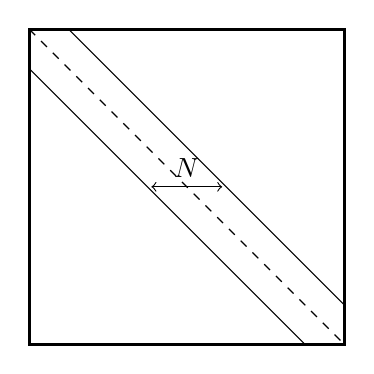
\begin{tikzpicture}
    \draw[very thick] (2,2)--(-2,2)--(-2,-2)--(2,-2)--cycle;
    \draw[dashed](-2,2)--(2,-2);
    \draw (-1.5,2)--(2,-1.5);
    \draw (-2,1.5)--(1.5,-2);

    \draw[<->] (-.45,0)--node[above]{$N$}(.45,0);
    \end{tikzpicture}
    \caption{An example of a banded matrix with width $N$, which has $N/2$ nonzero elements on both sides of the diagonal for each row.}
    \label{fig:banded}
\end{figure}

Let band segment $B_{z} = \set{z' : |z - z'| \le N/2}$.
The transition probabilities are then given by
\begin{equation}
    p(z_t \mid z_{t-1}) = \frac{[\theta]_{z_{t-1},z_{t}} + \phi(\bu_{z_{t-1}})^\top \phi(\bv_{z_{t}})}{Z_{z_{t-1}}},
\end{equation}
with normalizing constants
\begin{equation}
\begin{aligned}
Z_{z_{t-1}}
&= \sum_{z_{t}} [\theta]_{z_{t-1},z_{t}} + \phi(\bu_{z_{t-1}})^\top \phi(\bv_{z_{t}})\\
&= \sum_{z_{t}\in B_{z_{t-1}}} [\theta]_{z_{t-1},z_{t}} + 
    \phi(\bu_{z_{t-1}})^\top \sum_{z_t} \phi(\bv_{z_{t}}).
\end{aligned}
\end{equation}
The normalization constant for each starting state $Z_{z_{t-1}}$ can be computed in time $O(N)$.

This allows us to perform inference quickly.
We can use the above to rewrite the score matrix $\Psi_t \propto \theta + UV^\top$, which turns the inner loop of Eqn.~\ref{eqn:hypergraph-update-kernel-matrix} (specialized to HMMs) into
\begin{equation}
    \label{eqn:hmm-band-update}
    \alpha_t = \Psi_t\beta_{t+1} \propto (\theta + UV^\top)\beta_{t+1} = \theta\beta_{t+1} + U(V^\top \beta_{t+1}),
\end{equation}
omitting constants (i.e. emission probabilities and normalizing constants).
Since $\theta$ is banded, the banded matrix-vector product $\theta\beta_t$ takes time $O(LN)$.
This update, in combination with the low-rank product, takes $O(LN)$ time total. Each update in the hypergraph marginalization algorithm is now 3 matrix-vector products costing $O(LN)$ each, preserving the runtime of inference.

\section{Music Results}
\label{sec:full-music}
The full results on the polyphonic music modeling task can be found in Tbl.~\ref{tbl:full-music}, with additional models for comparison.
Aside from the RNN-NADE~\citep{polyphonic}, which models the full joint distribution of notes as well as temporal dependencies;  autoregressive neural R-Transformer~\citep{rtransformer} (as reported by \citet{betalstm}) and LSTM~(as reported by \citet{flow}); latent continuous LV-RNN \citep{nasmc} and SRNN \citep{srnn}; and latent discrete TSBN \citep{tsbn} and the baseline HMM; we additionally include the autoregressive Seq-U-Net \citet{sequnet}, the continuous latent STORN \citep{storn}, DMM \citep{dmm} and LNF \citep{flow}.

\begin{table}[t]
\centering
\begin{tabular}{lcccc}
\toprule
Model       & Nott & Piano & Muse & JSB \\
\midrule
%RNN      & 4.46       & 8.37        & 8.13       & 8.71          \\ 
%\midrule 
RNN-NADE & 2.31  & 7.05        & \textbf{5.6}        & 5.19          \\
Seq-U-Net & 2.97 & \textbf{1.93} & 6.96 & 8.173 \\
R-Transformer & \textbf{2.24} & 7.44 & 7.00 & 8.26 \\
LSTM  & 3.43 & 7.77   & 7.23 & 8.17     \\
STORN    & 2.85       & 7.13        &  6.16       & 6.91  \\
LV-RNN    & 2.72       & 7.61        & 6.89       &\textbf{ 3.99}\\
SRNN     & 2.94       & 8.2         & 6.28       & 4.74          \\
DMM     & 2.77 &    7.83 &  6.83 &  6.39 \\
LNF  & 2.39  & 8.19 & 6.92  & 6.53    \\
%AF / AF   & \textbf{2.39}  & 8.19 & 6.92  & 6.53    \\
%AF / SCF  & 2.56  & 8.26  & 6.95  & 6.64    \\
%IAF / SCF & 2.54  &  8.25 & 7.06  & 6.59    \\ 
\midrule
TSBN     & 3.67       & 7.89        & 6.81       & 7.48          \\
HMM &  2.43 & 8.51 & 7.34 & 5.74 \\
LHMM & 2.60 & 8.89 & 7.60 & 5.80 \\
\bottomrule
\end{tabular}
\caption{\label{tbl:full-music}
Polyphonic music negative log-likelihood, measured in nats.
The HMM models have $\mcL=2^{11}$ states and the LHMM has rank $N=2^{9}$, a 4:1 state:rank ratio.
}
\end{table}

\begin{figure*}[!tp]
  \centering
  \begin{subfigure}[t]{0.45\textwidth}
  \centering
  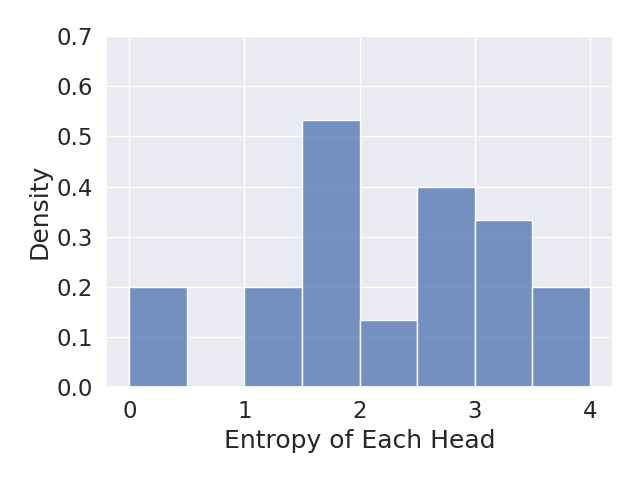
\includegraphics[width=0.9\textwidth]{imgs/softmax/entropy.png}
  \caption{Softmax Kernel $K_\SM$}
  \end{subfigure}
  \begin{subfigure}[t]{0.45\textwidth}
  \centering
  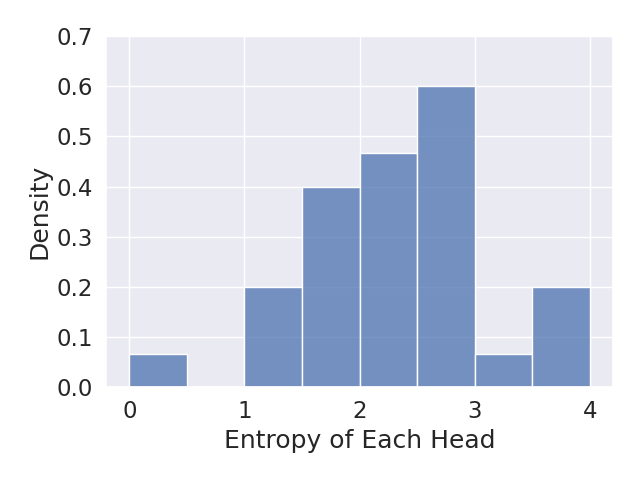
\includegraphics[width=0.9\textwidth]{imgs/rff/entropy.png}
  \caption{Linearized Kernel $K$}
  \end{subfigure}
  \caption{\label{fig:example_production}Histogram of entropies of $P(B\ C\mid A)$. The average entropy is 2.26 for softmax kernel and 2.34 for linearized kernel. We use $|\mcN|=30$, $|\mcP|=60$, and $N=16$ for linearized kernel.}
\end{figure*}
\section{PCFG Analysis}
\begin{table}[!htp]
\centering
\begin{tabular}{@{}ccccr@{}}
\toprule
\multicolumn{4}{c}{Kernel for $B\ C $} & \multirow{2}{*}{PPL}\\
\cmidrule{1-4}
$\mcN\times \mcN$ & $\mcN\times\mcP$  & $\mcP\times\mcN$ & $\mcP\times\mcP$ \\
\midrule
  SM & SM & SM & SM & 243.19\\
  $K$ & SM & SM & SM & 242.72\\
  $K$ & $K$ & $K$ & SM &  259.05 \\
  $K$ & $K$ & $K$ & $K$ & 278.60 \\
\bottomrule
\end{tabular}
\caption{\label{tbl:cky-ablation}Model perplexities evaluated on the validation set of \textsc{Ptb}. Here we use $|\mcN|=30$, $|\mcP|=60$, and $N=16$ features for linearized kernel. SM denotes the use of softmax kernels, while $K$ is an efficiently linearizable kernel.}
\end{table}

Figure~\ref{fig:example_production} shows the entropy distribution of the production rules $H(P(B\ C | A))$ for both using softmax kernel and the approximation. The average entropies of the two distributions are close. Besides, under this setting, $P(B\ C \in \mcN \times \mcN| A)$ are close for both kernels as well (softmax 0.20, linear 0.21), eliminating the possibility that the kernel model simply learns to avoid using $B\ C \in \mcN \times \mcN$ (such as by using a right-branching tree).

In Table~\ref{tbl:cky-ablation}, we consider the effects of the mixed kernel parameterization, i.e. of replacing the softmax kernel with a linearizable kernel. In particular, we consider different combinations of preterminal / nonterminal tails $B\ C\in \mcN\times\mcN$, $B\ C\in \mcN\times\mcP$, $B\ C\in \mcP\times\mcN$, and $B\ C\in \mcP\times\mcP$ (our main model only factorizes nonterminal / nonterminal tails). Table~\ref{tbl:cky-ablation} shows that we get the best perplexity when we only use $K$ on $B\ C\in \mcN\times\mcN$, and use softmax kernel $K_\SM$ for the rest of the space. This fits with previous observations that when the label space $|\mcL|$ is large, a model with a very small rank constraint hurts performance.\footnote{In this particular ablation study, the size of $\mcN\times\mcN$ is only one-ninth of the total state space size $\{\mcN \cup \mcP\}\times \{\mcN \cup \mcP\}$.}

%\section{\label{sec:pcfgvismore} PCFG Visualizations}
%TODO

\section{Potential Negative Impact}
\label{sec:impact}
While work on interpretable and controllable models is a step towards machine that can more easily be understood by and interact with humans, introducing external-facing components leaves models possibly more vulnerable to adversarial attacks. In particular, the interpretations (in conjunction with the predictions) afforded by interpretable models may be attacked \citep{adv-interp}. Additionally, models with simple dependencies may be easier for adversaries to understand and then craft attacks for \citep{Zhang2021LabelFA,adv-phmm}.
\end{document}


